\input{../../preamble2.tex}
\usepackage{tocloft}
\setlength{\cftsubsecnumwidth}{2.8em}
\begin{document}

\tableofcontents
\newpage

\section{Сформулируйте и докажите теорему о единственности предела сходящейся последовательности.}

\begin{theorem}[О единственности предела сходящейся последовательности]
  Любая сходящаяся последовательность имеет единственный предел.
\end{theorem}
\begin{proof}[][Аналитическое доказательство]
  Пусть $\{x_{n}\} $ --- сходящаяся последовательность (\textbf{опр.\ref{опр: сходящаяся последовательность}}) . \\
  Рассуждаем методом от противного. Пусть последовательность $\{x_{n}\} $ имеет более одного предела. \vspace{-\topsep}
  \begin{gather*}
    \lim_{n \to \infty} x_n = a \qquad \lim_{n \to \infty} x_n = b \qquad a \neq b 
  \end{gather*} \vspace{-2\topsep}
  \begin{gather}
    \lim_{n \to \infty} x_n = a \iff (\forall \varepsilon_1 > 0)(\exists N_1(\varepsilon_1) \in \N)\colon (\forall n > N_1(\varepsilon_1) \Rightarrow |x_{n} - a| < \varepsilon_1) \\
    \lim_{n \to \infty} x_n = b \iff (\forall \varepsilon_2 > 0)(\exists N_2(\varepsilon_2) \in \N)\colon (\forall n > N_2(\varepsilon_2) \Rightarrow |x_{n} - b| < \varepsilon_2)  
  \end{gather} 
  Выберем $N= \max \{N_1\left( \varepsilon_1 \right); N_2\left( \varepsilon_2 \right) \}$. \\[1ex]
  Пусть $\displaystyle \varepsilon = \varepsilon_1 = \varepsilon_2 = \frac{|b - a|}{3}$
  \begin{gather*}
    \begin{aligned}
      3 \varepsilon &= |b - a| = |b - a + x_{n} - x_{n}| = \\
      &= |(x_{n} - a) - (x_{n} - b)| \le |x_{n} - a| + |x_{n} - b| < \varepsilon_1 + \varepsilon_2 = 2 \varepsilon
    \end{aligned}\ \Rightarrow\ 3 \varepsilon < 2 \varepsilon
  \end{gather*}
  Противоречие. Значит, предположение не является верным $\implies$ последовательность $\{x_{n}\}$ имеет единственный предел, то есть $a=b\ \lim\limits_{n \to \infty} x_n = a$.
\end{proof}

\begin{proof}[][Геометрическое доказательство]
  Нельзя уложить бесконечное число членов последовательности $\{x_{n}\}$ в две непересекающиеся окрестности.\\[2ex]
  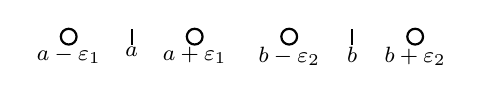
\begin{tikzpicture}[>=latex, scale=0.4, thick]
    \tkzInit[xmin=0, xmax=14, ymin=0, ymax=0]
    \tkzDrawX[very thick] \tkzGrid
    \draw (2, 0) node[below]{\footnotesize $a - \varepsilon_1$} circle (0.25);
    \draw (4, -0.25) -- (4, 0.25);
    \draw (6, 0) node[below]{\footnotesize $a + \varepsilon_1$} circle (0.25);
    \draw (9, 0) node[below]{\footnotesize $b - \varepsilon_2$} circle (0.25);
    \draw (11, -0.25) -- (11, 0.25);
    \draw (13, 0) node[below]{\footnotesize $b + \varepsilon_2$} circle (0.25);
    \node[below] at (4, 0) {\footnotesize $a$};
    \node[below] at (11, 0) {\footnotesize $b$};
  \end{tikzpicture}\\[2ex]
  $\begin{aligned}
    &S(a; \varepsilon_1)\\
    &S(b; \varepsilon_2)
  \end{aligned}$ \quad $\begin{aligned}
    &(1) \text{ бесконечное число членов последовательности } {\{x_n\}} \in S(a; \varepsilon_1). \\
    &(2) \text{ бесконечное число членов последовательности } {\{x_n\}} \in S(b; \varepsilon_2).
  \end{aligned}$
\end{proof}

\section{Сформулируйте и докажите теорему об ограниченности сходящейся последовательности.}

\begin{theorem}[Об ограниченности сходящейся последовательности]
    Любая сходящаяся последовательность ограничена. 
  \end{theorem}
  
\begin{proof}
    По определению сходящейся последовательности (\textbf{опр.\ref{опр: сходящаяся последовательность}})
    \vspace{-2pt}
    \begin{gather*}
         \lim_{n \to \infty} x_n = a \iff (\forall \varepsilon > 0)(\exists N(\varepsilon)\in \N)\colon (\forall n > N(\varepsilon)\ \Rightarrow\ |x_{n} - a| < \varepsilon).
    \end{gather*}
    Выберем в качестве $M = \max \{|x_{1}|, |x_2|, \ldots, |x_n|, |a - \varepsilon|, |a + \varepsilon|\}$. \\
    Тогда для $\forall n \in \N$ будет верно $|x_{n}| \le M$ -- это и означает, что $\{x_{n}\}$ --- ограничена.
\end{proof}
\newpage
\section{Сформулируйте и докажите теорему о локальной ограниченности функции, имеющей конечный предел.}
\begin{theorem}[О локальной ограниченности функции, имеющей конечный предел]
  Функция, имеющая конечный предел, локально ограничена.
\end{theorem}
\begin{proof} 
  \[
    \lim_{x \to x_0} f(x) = a\ \iff (\forall \varepsilon > 0)(\exists \delta(\varepsilon) > 0)\colon (\forall x \in \mathring{S}(x_0; \delta)\ \Rightarrow\ |f(x) - a| < \varepsilon)
  \]
  Распишем: \vspace{-\topsep}
  \begin{gather*}
    \begin{aligned}
      - \varepsilon < &f(x) - a < \varepsilon \\
      a - \varepsilon < &f(x) < a + \varepsilon
    \end{aligned}\qquad \forall  x \in \mathring{S}(x_0; \delta)
  \end{gather*}
  Выберем $M = \max \{|a - \varepsilon|; |a + \varepsilon|\}$.\quad Тогда $|f(x)| \le  M,\ \forall  x \in  \mathring{S}(x_0; \delta)$.
\end{proof}

\section{Сформулируйте и докажите теорему о сохранении функцией знака своего предела.}
\begin{theorem}[О сохранении функцией знака своего предела]\hlabel{о сохранении функцией знака своего предела}
  Если $\lim\limits_{x \to x_0} f(x) = a \ne 0$, то $\exists\ \mathring{S}(x_0; \delta)$ такая, что функция в ней сохраняет знак своего предела. \vspace{-\topsep}
  \begin{gather*}
  \text{Кратко:\quad Если} \lim_{x \to x_0} f(x) = a \ne 0\ \longrightarrow\ 
  \begin{aligned}
    a > 0\ \Rightarrow\ f(x) > 0 \\
    a < 0\ \Rightarrow\ f(x) < 0
  \end{aligned}\quad
  \forall x \in \mathring{S}(x_0; \delta)
  \end{gather*} 
\end{theorem}
\begin{proof}
  $\bullet$ Пусть $a > 0$. Выберем  $\varepsilon = a > 0$.
  \begin{gather*}
    \lim_{x \to x_0} f(x) = a \iff \big(\forall \varepsilon = a > 0\big)\big(\exists \delta(\varepsilon) > 0\big)\colon \big(\forall x \in \mathring{S}(x_0; \delta)\ \Rightarrow\
    |f(x)- a| < \varepsilon = a \big) 
  \end{gather*}
  Распишем: \vspace{-\topsep}
  \begin{gather*}
    -a < f(x) - a < a\ \Rightarrow\ \boxed{0 < f(x) < 2a}\quad \forall x \in \mathring{S} (x_0; \delta)
  \end{gather*}
  Знаки у функции $f(x)$ и числа $a$ --- одинаковые, <<$+$>>. \\[2ex]
  $\bullet$ Пусть $a < 0$. Выберем  $\varepsilon = -a > 0$.
  \begin{gather*}
    \lim_{x \to x_0} f(x) = a \iff \big(\forall \varepsilon = -a > 0\big)\big(\exists  \delta(\varepsilon) > 0\big)\colon \big(\forall x \in \mathring{S}(x_0; \delta)\ \Rightarrow\
    |f(x) - a| < \varepsilon = -a\big) 
  \end{gather*}
  Распишем: \vspace{-\topsep}
  \begin{gather*}
    a < f(x) - a < -a\ \Rightarrow\ \boxed{2a < f(x) < 0}\quad \forall x \in \mathring{S} (x_0; \delta)
  \end{gather*}
  Знаки у функции $f(x)$ и числа  $a$ --- одинаковые, <<$-$>>.\\[2ex]
  Значит, $f(x)$ сохраняет знак своего предела $\forall x \in \mathring{S}(x_0; \delta)$. 
  \begin{center}
    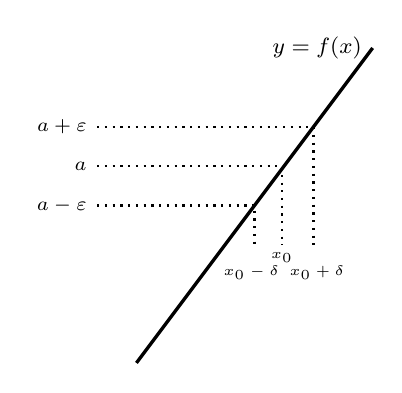
\begin{tikzpicture}[>=latex, thick, scale=0.5]
      \tkzInit[xmin=-2, xmax=8, ymin=-3, ymax=5]
      \tkzDrawX \tkzDrawY
      \draw[very thick] (1, -3) -- (7, 5) node[left]{\footnotesize $y=f(x)$};
      \draw[dotted] (0, 1) node[left]{\scriptsize $a - \varepsilon$} -| (4, 0) node[below=4pt]{\tiny $x_0 - \delta\ $};
      \draw[dotted] (0, 2) node[left]{\scriptsize $a$} -| (4.7, 0) node[below=-1pt]{\tiny $x_0$};
      \draw[dotted] (0, 3) node[left]{\scriptsize $a + \varepsilon$} -| (5.5, 0) node[below=4pt]{\tiny $\ x_0 + \delta$};
    \end{tikzpicture}\\
    $\lim\limits_{x \to x_0} f(x) = a > 0\ \Rightarrow\ \forall x \in \mathring{S}(x_0; \delta)\colon f(x) > 0$
  \end{center}
\end{proof}

\begin{corollary} \hlabel{Сл4}
  Если функция $y = f(x)$ имеет предел в точке  $x_0$ и знакопостоянна в $\mathring{S}(x_0; \delta)$, тогда её предел не может иметь с ней противоположные знаки.
\end{corollary} 

\section{Сформулируйте и докажите теорему о предельном переходе в неравенстве.}

\begin{theorem}[О предельном переходе в неравенстве]\hlabel{Предельный переход в неравенстве}
  Пусть существуют конечные пределы функций $f(x)$ и  $g(x)$ в точке $x_0$ и $\forall x \in \mathring{S}(x_0; \delta)$ верно $f(x) < g(x)$. Тогда $\forall x \in \mathring{S}(x_0; \delta)$ имеет место неравенство $\lim\limits_{x \to x_0} f(x) \le \lim\limits_{x \to x_0} g(x)$.
\end{theorem}
\begin{proof}
  По условию $f(x) < g(x), \forall x \in \mathring{S}(x_0; \delta)$. \\
  Введём функцию $F(x) = f(x) - g(x) < 0, \forall x \in \mathring{S}(x_0; \delta)$. \\
  Так как $f(x)$ и $g(x)$ имеют конечные пределы в точке $x_0$, то и функция $F(x)$ имеет конечный предел в точке $x_0$ (как разность $f(x)$ и $g(x)$).\\
  По следствию \textbf{\ref{Сл4}} $\implies \lim\limits_{x \to x_0} F(x) \le 0$ \\
  Подставим $F(x) = f(x) - g(x)$:
  \begin{gather*}
    \lim_{x \to x_0} \big( f(x) - g(x) \big) \le 0\ \Rightarrow\ \lim_{x \to x_0} f(x) - \lim_{x \to x_0} g(x) \le 0\ \Rightarrow\ \lim_{x \to x_0} f(x) \le \lim_{x \to x_0} g(x)\\
    \forall x \in \mathring{S}(x_0; \delta) 
  \end{gather*}
\end{proof}
\newpage
\section{Сформулируйте и докажите теорему о пределе промежуточной функции.}
\begin{theorem}[О пределе промежуточной функции]\hlabel{о пределе промежуточной функции}
  Пусть существуют конечные пределы функций $f(x)$ и $g(x)$ в точке $x_0$.\\
  $\lim\limits_{x \to x_0} f(x) = a$, $\lim\limits_{x \to x_0} g(x) = a$ и $\forall x \in \mathring{S}(x_0; \delta)$ верно неравенство $f(x) \le h(x) \le g(x)$. Тогда существует $\lim\limits_{x \to x_0} h(x) = a$.
\end{theorem}
\begin{proof}
  По условию: 
  \begin{align*}
    &\lim_{x \to x_0} f(x) = a \iff \big(\forall \varepsilon > 0\big)\big(\exists \delta_1(\varepsilon) > 0\big)\colon \big(\forall x \in \mathring{S}(x_0; \delta_1)\ \Rightarrow\ |f(x) - a| < \varepsilon\big) \tag{1} \\
    &\lim_{x \to x_0} g(x) = a \iff \big(\forall \varepsilon > 0\big)\big(\exists \delta_2(\varepsilon) > 0\big)\colon \big(\forall x \in \mathring{S}(x_0; \delta_2)\ \Rightarrow\ |g(x) - a| < \varepsilon\big) \tag{2}
  \end{align*}
  Выберем $\delta_0 = \min \{\delta_1; \delta_2; \delta\}$, тогда (1), (2) и $f(x) \le h(x) \le g(x)$ верны одновременно $\forall x \in \mathring{S}(x_0; \delta_0)$.
  \begin{align*}
    \left. \begin{aligned}
    (1) \quad a - \varepsilon < &f(x) < a + \varepsilon \\
    (2) \quad a - \varepsilon < &g(x) < a + \varepsilon \\
    f(x) \le &h(x) \le g(x)
    \end{aligned}\right\} &\Rightarrow\ a - \varepsilon < f(x) \le h(x) \le g(x) < a + \varepsilon\ \Rightarrow \\
    &\Rightarrow\ \forall x \in \mathring{S}(x_0; \delta_0) \quad a - \varepsilon < h(x) < a + \varepsilon
  \end{align*} 
  В итоге: \vspace{-\topsep}
  \begin{gather*}
    \big(\forall \varepsilon > 0\big)\big(\exists \delta_0(\varepsilon) > 0\big)\colon \big(\forall x \in \mathring{S}(x_0; \delta_0)\ \Rightarrow\ |h(x) - a| < \varepsilon\big) \\
    \Downarrow \\
    \text{По определению предела } (\textbf{\ref{sec: предел функции}})\colon \lim_{x \to x_0} h(x) = a
  \end{gather*}
\end{proof}

\section{Сформулируйте и докажите теорему о пределе произведения функций.}

\begin{theorem}[О пределе произведения функций]
  Предел произведения функций равен произведению пределов этих функций.
  \begin{gather*}
    \lim_{x \to x_0} \big(f(x) \cdot g(x)\big) = \lim\limits_{x \to x_0} f(x) \cdot \lim\limits_{x \to x_0} g(x)
  \end{gather*}
\end{theorem}
\begin{proof}
  Пусть: $(1)\ \lim\limits_{x \to x_0} f(x) = a \qquad (2)\ \lim\limits_{x \to x_0} g(x) = b$ \\[1ex]
  По теореме \textit{о связи функции, её предела и бесконечно малой функции} (\textbf{Т.\ref{О связи функции, её предела и б.м.ф.}}):
  \begin{align*}
    (1)\colon &f(x) = a + \alpha(x) \text{, где } \alpha(x) \text{ --- б.м.ф. при } x\to x_0 \\
    (2)\colon &g(x) = b + \beta(x) \text{, где } \beta(x) \text{ --- б.м.ф. при } x\to x_0
  \end{align*}
  Рассмотрим $f(x) \cdot g(x)$:
  \begin{align*}
    f(x) \cdot g(x) = \big(a + \alpha(x)\big)\cdot \big(b + \beta(x)\big) = ab + \underbrace{a \cdot \beta(x) + \alpha (x)\cdot b + \alpha(x) \cdot \beta(x)}_{\gamma(x)} = ab + \gamma(x) 
  \end{align*}
  По следствиям из теоремы \textbf{Т.\ref{О связи функции, её предела и б.м.ф.}}:
  \begin{align*}
    a \cdot \beta(x) &= \text{б.м.ф. при } x \to x_0\qquad (\textbf{сл.\ref{сл: произведение б.м.ф и константы}}) \\ 
    b \cdot \alpha(x) &= \text{б.м.ф. при } x \to x_0\qquad (\textbf{сл.\ref{сл: произведение б.м.ф и константы}}) \\ 
    \alpha(x) \cdot \beta(x) &= \text{б.м.ф. при } x \to x_0\qquad (\textbf{сл.\ref{сл: произведение б.м.ф}})
  \end{align*}
  По теореме \textit{о сумме конечного числа б.м.ф.} (\textbf{Т.\ref{о сумме конечного числа б.м.ф.}}):
  \begin{gather*}
    \gamma(x) = \text{б.м.ф. при } x \to x_0
  \end{gather*}
  Распишем предел произведения:
    \begin{align*}
      \lim_{x \to x_0} \big(f(x) \cdot g(x)\big) &= \lim_{x \to x_0} \big(ab + \gamma(x)\big) = \lim_{x \to x_0} ab + \lim_{x \to x_0} \gamma(x) = \\
      &= ab + 0 = ab = \lim\limits_{x \to x_0} f(x) \cdot \lim\limits_{x \to x_0} g(x)
    \end{align*}
\end{proof}

\section{Сформулируйте и докажите теорему о пределе сложной функции.}

\begin{theorem}[О пределе сложной функции]
  Если функция $y = f(x)$ имеет предел в точке  $x_0$ равный $a$, то функция  $\varphi(y)$ имеет предел в точке $a$, равный $c$, тогда сложная функция  $\varphi\big(f(x)\big)$ имеет предел в точке $x_0$ равный $c$. Кратко: \vspace{-\topsep}
  \begin{gather*}
    \left. \begin{aligned}
      &y = f(x) \\
      \lim\limits_{x \to x_0} &f(x) = a \\
      \lim\limits_{y \to a}\ &\varphi(y) = c \\
    \end{aligned}\right\}\ \Rightarrow\ \lim\limits_{x \to x_0} \varphi\big(f(x)\big) = c
  \end{gather*}
\end{theorem}
\begin{proof}
  По условию: \vspace{-4pt}
  \begin{gather*}
    \lim_{y \to a} \varphi(y) = c \iff \big(\forall \varepsilon > 0\big)\big(\exists \delta_1 > 0\big)\colon \big(\forall y\colon 0 < |y-a| < \delta_1\ \Rightarrow\ |\varphi(y) - c| < \varepsilon\big) \tag{1}
  \end{gather*}
  Выберем в качестве $\varepsilon$ в пределе найденное $\delta_1\ (\varepsilon = \delta_1)$: \[
    \lim_{x \to x_0} f(x) = a \iff \big(\forall \delta_1 > 0\big) \big(\exists \delta_2 > 0\big)\colon \big(\forall x\colon 0 < |x - x_0| < \delta_2\ \Rightarrow\ |f(x) - a| < \delta_1\big) \tag{2} 
  \]
  В итоге: \vspace{-\topsep} \[
  \big(\forall \varepsilon > 0\big)\big(\exists \delta_2 > 0\big)\colon \big(\forall x\colon 0 < |x - x_0| < \delta_2\ \Rightarrow\ \left|\varphi\big(f(x)\big) - c\right| < \varepsilon\big)
  \] 
  Что равносильно: \vspace{-0.8\topsep} \[
  \lim\limits_{x \to x_0} \varphi\big(f(x)\big) = c
  \] 
\end{proof}

\section{Докажите, что $\lim\limits_{x \to 0}\frac{\sin x}{x} = 1$.}

\begin{theorem} 
  \[
    \boxed{\lim_{x \to 0} \frac{\sin x}{x} = 1}
  \]  
\end{theorem}
\begin{proof}
  1. Рассмотрим $\lim\limits_{x \to 0+} \dfrac{\sin x}{x} = 1$, $\lim\limits_{x \to 0-} \dfrac{\sin x}{x} = 1\ \Rightarrow\ \lim\limits_{x \to 0} \dfrac{\sin x}{x} = 1$  \\[1ex]
  2. Пусть $x$ --- угол в радианах, $x \to 0+,\ x \in \left(0; \dfrac{\pi}{2}\right)$.\\
% рисунок
  Окружность $R = 1$.\\[1ex]
  3. Отложим $\angle x\colon$ вершина совпадает с точкой $O(0;0)$, 1 сторона --- с положительным направлением $OX$, $A(1;0)$.\\
  $K$ --- точка пересечения $\angle x$ и окружности. \\
  $l$ --- касательная к окружности в точке $A$, пересекает $OK$. \\
  $KH \perp OA$, $H \in OA$.\\[1ex] 
  4. Рассмотрим $\triangle OKH$: $OK = 1 = R_{\text{окр.}}\quad \sin x = \dfrac{KH}{OK} = KH$. \\[1ex] 
  5. Рассмотрим $\triangle OLA$: $OA = 1 = R_{\text{окр.}}\quad \tg x = \dfrac{LA}{OA} = LA$. \\[1ex]
  6. Из геометрических построений:
  \begin{flalign*}
    & S_{\triangle OKA} < S_{\text{сек. } OKA} < S_{\triangle OLA} &\\
    & S_{\triangle OKA} = \frac{1}{2}\cdot OA \cdot KH = \frac{1}{2}\cdot \sin x = \frac{\sin x}{2}  &\\
    & S_{\text{сек. } OKA} = \frac{1}{2}\cdot OA \cdot OK \cdot \overset{\frown}{KA} = \frac{1}{2}\cdot \overset{\frown}{KA} = \frac{1}{2} \cdot x = \frac{x}{2} &\\
    & S_{\triangle OLA} = \frac{1}{2}\cdot OA \cdot LA = \frac{1}{2} \cdot 1 \cdot \tg x = \frac{\tg x}{2} &
  \end{flalign*} \vspace{-15\topsep}
  \begin{flushright}
    \begin{tikzpicture}[>=latex, thick, scale=1.7]
      \tkzInit[xmin=-1.3, xmax=1.5, ymin=-1.5, ymax=1.2]
      \tkzDrawX[label={$\cos x$}] \tkzDrawY[label={$\sin x$}]
      \tkzDefPoint(0, 0){O}
      \tkzDefPoint(1, 0){A}
      \tkzDefPoint(3/4, 0){H}
      \tkzDefPoint(1, {tan(3/4)}){L}
      \tkzDefPoint(3/4, {sin(3/4)}){K}
      \tkzDrawPoint[size = 3pt](K)
      \draw[very thick] (0, 0) node[below left]{$0$} circle (1);
      \tkzLabelAngle[pos=1/3, font=\scriptsize](A,O,K){$x$}
      \tkzMarkAngle[mark=none, thin, size=1/4](A,O,K)
      \draw[very thick] (O) node[below right]{\scriptsize $O$} -- (L) node[right]{\scriptsize $L$};
      \draw[very thick, add=1.2 and 0.7] (A) node[below right]{\scriptsize $A$} to (L) node[right]{\scriptsize $l$};
      \draw[dotted, very thick] (K) node[above=2pt]{\scriptsize $K$} -- (H) node[below]{\scriptsize $H$};
      \tkzMarkRightAngle[mark=none, thin, size=0.125](O,H,K)
      \draw[very thick] (A) -- (K);
    \end{tikzpicture}
  \end{flushright} \vspace{-5\topsep}
  \begin{flalign*}
    & \frac{\sin x}{2} < \frac{x}{2} < \frac{\tg x}{2} \quad \Big| \cdot 2 &\\[1ex]
    & \begin{rcases}
      \sin x < x < \tg x \\
      x \to 0+\ \Rightarrow\ \begin{cases}
        \sin x > 0 \\
        \tg x > 0
      \end{cases}
    \end{rcases}\ \Rightarrow\ \sin x < x < \tg x \quad | : \sin x & \\[1ex]
    & 1 < \frac{x}{\sin x} < \frac{1}{\cos x}\ \Rightarrow\ \cos x < \frac{\sin x}{x} < 1 &
  \end{flalign*}
   По теореме \textit{о предельном переходе в неравенстве} (\textbf{Т.\ref{Предельный переход в неравенстве}}): \[
   \lim_{x \to 0+} \cos x \le \lim_{x \to 0+} \frac{\sin x}{x} \le 1
   \] 
   По теореме \textit{о промежуточной функции} (\textbf{Т.\ref{о пределе промежуточной функции}}): \[
    \lim_{x \to 0+} \cos x = 1\ \Rightarrow\ \lim_{x \to 0+} \frac{\sin x}{x} = 1 
   \] 
   Аналогично для $\lim\limits_{x \to 0-} \dfrac{\sin x}{x} = 1$.\\
   По теореме \textit{о существовании предела функции в точке} (\textbf{Т.\ref{существование предела в точке}}): \[
   \lim_{x \to 0+} \frac{\sin x}{x} = \lim_{x \to 0-} \frac{\sin x}{x} = 1\ \Rightarrow\ \lim_{x \to 0} \frac{\sin x}{x} = 1
   \] 
\end{proof}

\section{Сформулируйте и докажите теорему о связи функции, ее предела и бесконечно малой.}

\begin{theorem}[О связи функции, её предела и бесконечно малой]\hlabel{О связи функции, её предела и б.м.ф.}
  Функция $y = f(x)$ имеет конечный предел в точке  $x_0$ тогда и только тогда, когда её можно представить в виде суммы предела и некоторой бесконечно малой функции.
  \begin{gather*}
    \lim_{x \to x_0} f(x) = a \iff f(x) = a + \alpha(x), \text{где } \alpha(x) - \text{б.м.ф при } x \to x_0
  \end{gather*}
\end{theorem}
\begin{proof}[][Необходимость]
  \textbf{Дано}: $\displaystyle \lim_{x \to x_0} f(x) = a$ \\
  \textbf{Доказать}: $\displaystyle f(x) = a + \alpha(x), \text{где } \alpha(x) \text{ --- б.м.ф. при } x \to  x_0 $ \\[1ex]
  По условию: \[
    \lim_{x \to x_0} f(x) = a \iff \big(\forall \varepsilon > 0\big)\big(\exists \delta > 0\big)\colon \big(\forall x \in \mathring{S}(x_0; \delta)\ \Rightarrow\ |f(x) - a| < \varepsilon\big)  
  \]
  Обозначим $f(x) - a = \alpha(x)$, тогда: \[
    \lim_{x \to x_0} f(x) = a \iff \big(\forall \varepsilon > 0\big)\big(\exists \delta > 0\big)\colon \big(\forall x \in \mathring{S}(x_0; \delta)\ \Rightarrow\ |\alpha(x)| < \varepsilon\big)  
  \]
  По определению бесконечно малой функции (\textbf{опр.\ref{опр: б.м.ф.}}) $\alpha(x)$ --- б.м.ф. \\
  Из обозначения следует, что $f(x) = a + \alpha(x)$, где $\alpha(x)$ --- б.м.ф при $x \to x_0$.
\end{proof}
\begin{proof}[][Достаточность]
  \textbf{Дано}: $f(x) = a + \alpha(x), \text{где } \alpha(x) \text{ --- б.м.ф. при } x \to x_0$ \\
  \textbf{Доказать}: $\lim\limits_{x \to x_0} f(x) = a$ \\[1ex]
  По определению б.м.ф.: \[
    \lim_{x \to x_0} \alpha(x) = 0 \iff \big(\forall \varepsilon > 0\big)\big(\exists \delta > 0\big)\colon \big(\mathring{S}(x_0; \delta)\ \Rightarrow\ |\alpha(x)| < \varepsilon\big)
  \]
  С учётом введённого обозначения: \[
    \big(\forall \varepsilon > 0\big)\big(\exists \delta > 0\big)\colon \big(\mathring{S}(x_0; \delta)\ \Rightarrow\ |f(x) - a| < \varepsilon\big) \iff \lim_{x \to x_0} f(x) = a
  \]
\end{proof}
\begin{corollary}\hlabel{сл: произведение б.м.ф}
  Так как любая бесконечно малая функция локально ограничена, то произведение двух бесконечно малых функций есть бесконечно малая функция.
\end{corollary}
\begin{corollary}\hlabel{сл: произведение б.м.ф и константы}
  Произведение бесконечно малой функции на константу есть величина бесконечно малая.
\end{corollary}

\setcounter{equation}{0}
\section{Сформулируйте и докажите теорему о произведении бесконечно малой функции на ограниченную.}

\begin{theorem}[О произведении бесконечно малой функций на локально ограниченную]\hlabel{о произведении б.м.ф. на ограниченную}
  Произведение бесконечно малой функции на локальной ограниченную есть величина бесконечно малая.
\end{theorem}
\begin{proof}
  Пусть $\alpha(x)$ --- б.м.ф. при $x \to x_0$, а функция $f(x)$ при $x \to  x_0$ является локально ограниченной.\\
  \textbf{Доказываем, что}: $\alpha(x) \cdot f(x) = 0$\\
  По определению б.м.ф. (\textbf{опр.\ref{опр: б.м.ф.}}): \vspace{-\topsep}
  \begin{gather}
    \begin{aligned}
      &\lim_{x \to x_0} \alpha(x) = 0 
      \iff \left(\forall \varepsilon_1 = \frac{\varepsilon}{M} > 0\right)\big(\exists \delta_1 > 0\big)\colon \left(\forall x \in \mathring{S}(x_0; \delta_1) \Rightarrow\ |\alpha(x)| < \varepsilon_1 = \frac{\varepsilon}{M}\right)\\
      &M \in \R,\ M > 0
    \end{aligned}
  \end{gather}
  По определению локально ограниченной функции (\textbf{опр.\ref{опр: локально ограниченная функция}}):
  \begin{gather} 
    \exists M \in \R, M > 0,\quad \forall x \in  \mathring{S}(x_0; \delta_2)\ \Rightarrow\ |f(x)| < M
  \end{gather}
  Выберем $\delta = \min \{\delta_1; \delta_2\} $, тогда (1) и (2) верны одновременно. В итоге получаем:
  \begin{gather*}
    \big(\forall \varepsilon > 0\big)\big(\exists \delta > 0\big)\colon \left(\forall x \in \mathring{S}(x_0; \delta)\ \Rightarrow\ |\alpha(x) \cdot f(x)| = |\alpha(x)| \cdot |f(x)| < \frac{\varepsilon}{M} \cdot M = \varepsilon \right)
  \end{gather*}
  Тогда по определению бесконечно малой функции:
  \[
  \lim_{x \to x_0} \big(\alpha(x) \cdot f(x)\big) = 0
  \] 
\end{proof}
\setcounter{equation}{0}

\newpage
\section{Сформулируйте и докажите теорему о связи между бесконечно большой и бесконечно малой.}

\begin{theorem}[О связи бесконечно малой и бесконечно большой функции]
  Если $\alpha(x)$ --- бесконечно большая функция при $x \to x_0$, то $\dfrac{1}{\alpha(x)}$ --- бесконечно малая функция при $x \to x_0$.
\end{theorem}
\begin{proof}
  По условию $\alpha(x)$ --- б.б.ф. при $x \to x_0$. По определению б.б.ф. (\textbf{опр.\ref{опр: б.б.ф.}}):
  \begin{gather*}
    \lim_{x \to x_0} \alpha(x) = \infty \iff \big(\forall M > 0\big)\big(\exists \delta(M) > 0\big)\colon \big(\forall x \in \mathring{S}(x_0; \delta)\ \Rightarrow\ |\alpha(x)| > M\big)
  \end{gather*}
  Рассмотрим неравенство: \[
    |\alpha(x)| > M,\ \forall x \in \mathring{S}(x_0; \delta)
  \]
  Обозначим $\varepsilon = \dfrac{1}{M}$.
  \begin{gather*}
    |\alpha(x)| > M\ \Rightarrow\ \frac{1}{|\alpha(x)|} < \frac{1}{M}
   \ \Rightarrow\ \left| \frac{1}{\alpha(x)} \right| < \varepsilon
  \end{gather*}
  По определению б.м.ф. (\textbf{опр.\ref{опр: б.м.ф.}}):
  \begin{gather*}
    \lim\limits_{x \to x_0} \frac{1}{\alpha(x)} = 0\ \Rightarrow\ \frac{1}{\alpha(x)} \text{ --- б.м.ф при } x\to x_0
  \end{gather*}
\end{proof}

\section{Сформулируйте и докажите теорему о замене бесконечно малой на эквивалентную под знаком предела.}

\begin{theorem}[О замене функции на эквивалентную под знаком предела] 
  Предел отношения двух б.м.ф. (б.б.ф.) не изменится, если заменить эти функции на эквивалентные. Кратко: \[
  \begin{rcases}
    \alpha(x) \text{ и } \beta(x) \text{ --- б.м.ф. при } x \to x_0 \\
    \alpha(x) \sim \alpha_0(x) \\
    \beta(x) \sim \beta_0(x)
  \end{rcases}\ \Rightarrow\ 
  \lim_{x \to x_0} \frac{\alpha(x)}{\beta(x)} = \lim\limits_{x \to x_0}  \frac{\alpha_0(x)}{\beta_0(x)} 
  \] 
\end{theorem}
\begin{proof}
  Рассмотрим предел:
  \begin{align*}
    \lim_{x \to x_0} \frac{\alpha(x)}{\beta(x)} = \lim_{x \to x_0} \frac{\alpha(x) \cdot \alpha_0(x) \cdot \beta_0(x)}{\beta(x) \cdot \alpha_0(x) \cdot \beta_0(x)} &= \lim_{x \to x_0} \frac{\alpha(x)}{\alpha_0(x)} \cdot \lim_{x \to x_0} \frac{\beta_0(x)}{\beta(x)} \cdot \lim_{x \to x_0} \frac{\alpha_0(x)}{\beta_0(x)} = \\
   &= 1 \cdot 1 \cdot \lim_{x \to x_0} \frac{\alpha_0(x)}{\beta_0(x)}
  \end{align*}
\end{proof} 

\section{Сформулируйте и докажите теорему о необходимом и достаточном условии эквивалентности бесконечно малых.}

\begin{theorem}[Необходимое и достаточное условие эквивалентности бесконечно малых функций]
  Две бесконечно малые функции $\alpha(x)$ и $\beta(x)$ эквивалентны тогда и только тогда, когда их разность имеет более высокий порядок малости по сравнению с каждой из них.
  \begin{gather*}
    \alpha(x) \text{ и } \beta(x) \text{ --- б.м.ф при } x \to x_0 \\
    \alpha(x) \sim \beta(x) \text{ при } x\to x_0 \iff 
    \begin{matrix}
    \alpha(x) - \beta(x) = o\big(\alpha(x)\big) \\
    \alpha(x) - \beta(x) = o\big(\beta(x)\big)
    \end{matrix}
    \quad \text{при } x \to x_0
  \end{gather*}
\end{theorem}
\begin{proof}[][Необходимость]
  \textbf{Дано}: $\alpha(x) \text{ и } \beta(x) \text{ --- б.м.ф при } x \to x_0,\quad \alpha(x) \sim \beta(x) \text{ при }  x\to x_0$\\
  \textbf{Доказать}: $\alpha(x) - \beta(x) = o\big(\alpha(x)\big) \text{, при } x \to x_0$ \\
  Рассмотрим:
  \begin{align*}
    \lim_{x \to x_0} \frac{\alpha(x) - \beta(x)}{\alpha(x)} &= \lim_{x \to x_0} \left( 1 - \frac{\beta(x)}{\alpha(x)} \right) = 1 - \lim_{x \to x_0} \frac{\beta(x)}{\alpha(x)} = 1 - 1 = 0
  \end{align*}
  Аналогично доказывается, что $\alpha(x) - \beta(x) = o\big(\beta(x)\big)$ при $x\to x_0$.
\end{proof}
\begin{proof}[][Достаточность]
  \textbf{Дано}: $\alpha(x) - \beta(x) = o\big(\beta(x)\big) \text{ при } x \to x_0$ \\
  \textbf{Доказать}: $\alpha(x) \sim \beta(x) \text{ при } x \to x_0$ \\
  Рассмотрим:
  \begin{align*}
    &\lim_{x \to x_0} \frac{\alpha(x) - \beta(x)}{\beta(x)} = \lim_{x \to x_0} \left( \frac{\alpha(x)}{\beta(x)} - 1 \right) = \lim_{x \to x_0} \frac{\alpha(x)}{\beta(x)} - 1 = 0\ \Rightarrow \\
    &\Rightarrow\ \lim_{x \to x_0} \frac{\alpha(x)}{\beta(x)} = 1\ \Rightarrow\ \alpha(x) \sim \beta(x) \text{ при } x \to x_0 
  \end{align*}
\end{proof}

\newpage
\section{Сформулируйте и докажите теорему о сумме конечного числа бесконечно малых разных порядков.}

\begin{theorem}[О сумме бесконечно малых разного порядка] \hlabel{Сумма бмф разного порядка}
  Сумма бесконечно малых функций разных порядков малости эквивалентна слагаемому низшего порядка малости.
  \begin{gather*}
    \begin{rcases}
      \alpha(x), \beta(x) \text{ --- б.м.ф при } x \to x_0 \\
      \alpha(x) = o\big(\beta(x)\big) \text{ при } x \to x_0
    \end{rcases} 
    \implies \alpha(x) + \beta(x) \sim \beta(x) \text{, при } x \to x_0
  \end{gather*}
\end{theorem}
\begin{proof}
  Рассмотрим предел:
  \begin{align*}
    \lim_{x \to x_0} \frac{\alpha(x) + \beta(x)}{\beta(x)} &= \lim_{x \to x_0} \left( \frac{\alpha(x)}{\beta(x)} + 1 \right) = \lim_{x \to x_0} \left( \frac{\alpha(x)}{\beta(x)}\right) + 1 = 0 + 1 = 1
  \end{align*} 
\end{proof}

\begin{corollary}
  Сумма б.б.ф. разного порядка роста эквивалентна слагаемому высшего порядка роста. 
\end{corollary}

\section{Сформулируйте и докажите теорему о непрерывности суммы, произведения и частного непрерывных функций.}

\begin{theorem}
  Пусть функции: \[
    \begin{rcases*}
      y = f(x) \\
      y = g(x)
    \end{rcases*}
    \in C(x_0) \]
  Тогда:
  \begin{enumerate}
    \item $f(x) + g(x) \in C(x_0)$
    \item $f(x) \cdot g(x) \in C(x_0)$
    \item $\dfrac{f(x)}{g(x)} \in C(x_0),\ g(x) \ne 0$
  \end{enumerate}
\end{theorem}
\begin{proof}
  По определению непрерывной функции (\textbf{Т.\ref{опр: функция непрерывная в точке}}): 
  \begin{gather*} 
    \lim_{x \to x_0} f(x) = f(x_0) \\
    \lim_{x \to x_0} g(x) = g(x_0) 
  \end{gather*}
  Рассмотрим: 
  \begin{gather*}
    \lim_{x \to x_0} \big(f(x) + g(x)\big) = \lim_{x \to x_0} f(x) + \lim_{x \to x_0} g(x) = f(x_0) + g(x_0) \tag{1}\\
    \Updownarrow \\
    f(x) + g(x) \in C(x_0) \\[2ex]
    \lim_{x \to x_0} \big(f(x) \cdot g(x)\big) = \lim_{x \to x_0} f(x) \cdot \lim_{x \to x_0} g(x) = f(x_0) \cdot g(x_0) \tag{2} \\
    \Updownarrow \\
    f(x) \cdot g(x) \in C(x_0) \\[2ex]
    \lim_{x \to x_0} \frac{f(x)}{g(x)} = \frac{\lim\limits_{x \to x_0} f(x)}{\lim\limits_{x \to x_0} g(x)} = \frac{f(x_0)}{g(x_0)} \tag{3} \\
    \Updownarrow \\
    \frac{f(x)}{g(x)} \in C(x_0),\ g(x) \ne 0
  \end{gather*}
\end{proof}

\section{Сформулируйте и докажите теорему о непрерывности сложной функции.}

\begin{theorem}[О непрерывности сложной функции]
  Пусть функция $f(x)$ непрерывна в точке $x_0$, а $g(y)$ в точке $y_0$, причём $y_0 = f(x_0)$.\\
  Тогда сложная функция $F(x) = g\big(f(x)\big)$ непрерывна в точке $x_0$
\end{theorem}
\begin{proof}
  Так как $y=f(x) \in C(x_0)\ \Rightarrow\ \lim\limits_{x \to x_0} f(x) = f(x_0)$\\
  Так как $g(y) \in C(x_0)\ \Rightarrow\ \lim\limits_{y \to y_0} g(y) = g(y_0),\ y_0 = f(x_0)$\\
  Рассмотрим $\lim\limits_{x \to x_0} F(x) = \lim\limits_{x \to x_0} g\big(f(x)\big) \xlongequal{\text{Т.\ref{для непрерывности сложной функции}}} g\left(\lim\limits_{x \to x_0} f(x)\right) \xlongequal{\text{непр. } f} g\big(f(x_0)\big) = F(x_0)\ \Rightarrow$\\
  $\Rightarrow\ g\big(f(x)\big) \in C(x_0)$
\end{proof}

\newpage
\section{Сформулируйте и докажите теорему о сохранении знака непрерывной функции в окрестности точки.}

\begin{theorem}[О сохранении знака непрерывной функции в окрестности точки]
  Если функция $y=f(x)$ непрерывна в точке $x_0$ и $f(x_0) \ne 0$, то $\exists\ S(x_0)$, в которой знак значений функции совпадает со знаком $f(x_0)$.
\end{theorem}
\begin{proof}
  Так как $y=f(x)$ непрерывна в точке $x_0$, то $\lim\limits_{x \to x_0} f(x) = f(x_0)$.\\
  По теореме \textit{о сохранении функцией знака своего предела} (\textbf{Т.\ref{о сохранении функцией знака своего предела}}) $\Rightarrow\ \exists\ S(x_0)$, в которой знак значений функции совпадает со знаком $f(x_0)$.
\end{proof}
\begin{note}
  На экзамене требуется доказать также и теорему о сохранении функцией знака своего предела!
\end{note}

\section{Дайте определение функции, непрерывной в точке. Сформулируйте теорему о непрерывности элементарных функций. Докажите непрерывность функций $y = \sin x$, $y = \cos x$.}

\begin{definition}
  Функция $f(x)$, определённая в некоторой окрестности точки $x_0$, называется \textbf{непрерывной в} этой \textbf{точке} если: \[
    \exists \lim_{x \to x_0} f(x) = f(x_0)
  \]
\end{definition}
\begin{note}
  Множество непрерывных функций в точке $x_0$ обозначается $C(x_0)$. 
  \[
    f(x) \in C(x_0) \iff \text{ функция непрерывна в точке } x_0
  \] 
\end{note}
\begin{theorem}
  Основные элементарные функции непрерывны в области определения.
\end{theorem}
\begin{proof}
  $\bullet$ Докажем её для функций $y = \sin x$ и $y=\cos x$. \\
  1. Возьмём $y = \sin x,\ D_f \in \R$.
  \[ x_0 = 0\quad \lim\limits_{x \to 0} \sin x = \sin 0 = 0\ \Rightarrow\ y= \sin x \in C(0) \]
  2. Возьмём $\forall x_0 \in D_f \in \R$, $\Delta x$ --- приращение аргумента.
  \[ x = x_0 + \Delta x ,\ x \in D_f = \R \]
  3. Соответствующее приращение функции:
  \begin{align*}
    \Delta y &= f(x) - f(x_0) = y(x_0 + \Delta x) - y(x_0) = \sin(x_0 + \Delta x) - \sin(x_0) = \\
    &= 2\cdot \sin \frac{x_0 + \Delta x - x_0}{2}\cdot \cos \frac{x_0 + \Delta x + x_0}{2} = 2\cdot \sin \frac{\Delta x}{2}\cdot \cos \left( x_0 + \frac{\Delta x}{2} \right)
  \end{align*}
  4. По теореме \textit{о произведении б.м.ф. на ограниченную} (\textbf{Т.\ref{о произведении б.м.ф. на ограниченную}}):
  \begin{gather*}
    \lim\limits_{\Delta x \to 0} \Delta y = \lim\limits_{\Delta x \to 0} \left( 2\cdot \sin \frac{\Delta x}{2}\cdot \cos \left(x_0 + \frac{\Delta x}{2} \right) \right) = 0
  \end{gather*}
  5. $\sin \dfrac{\Delta x}{2}$ --- б.м.ф. при $\Delta x \to 0$ ?
  \[ \lim\limits_{\Delta x \to 0} \sin \frac{\Delta x}{2} = \sin 0 = 0\ \Rightarrow\ \sin \frac{\Delta x}{2} \text{ --- б.м.ф при } \Delta x \to 0 \]
  6. $\cos \left( x_0 + \dfrac{\Delta x }{2} \right)$ --- огр. функция?
    \[ \frac{\Delta x}{2} \to 0,\ \cos(x_0) \text{ --- огр.}\ \Rightarrow\ \left| \cos \left( x_0 + \frac{\Delta x}{2} \right) \right| \le 1 \text{ --- огр. функция} \]
  7. Так как $\lim\limits_{\Delta x \to 0} \Delta y = 0$ по определению непрерывной функции (\textbf{опр.\ref{опр: функция непрерывная в точке}}) $\Rightarrow\ y = \sin x$ непрерывна в точке $x_0$. \\
  8. Так как $x_0$ --- произвольная точка из области определения, то $y = \sin x$ непрерывна на всей области определения. \\[1ex]
  $\bullet\  \cos x\colon \Delta y = \cos(x_0 + \Delta x) - \cos (x_0)$.
\end{proof}
\begin{remark}
  Эта теорема доказывается для каждой из элементарных функций отдельно.
\end{remark}
\newpage
\section{Сформулируйте свойства функций, непрерывных на отрезке.}

\begin{theorem}[об ограниченности непрерывной функции (\textbf{Первая теорема Вейерштрасса})]
  Если функция $y=f(x)$ непрерывна на $[a, b]$, то она на этом отрезке ограничена.\\
  Кратко: \vspace{-\topsep}
  \begin{gather*}
    \big(f(x) \in C[a, b]\big)\ \Rightarrow\ \big(\exists\ M \in \R, M>0\big) \big(\forall x \in [a, b]\colon |f(x)| \le M\big)
  \end{gather*}
\end{theorem}
\begin{theorem}[о достижении непрерывной функции наибольшего и наименьшего значений (\textbf{Вторая теорема Вейерштрасса})]\hlabel{Вейерштрасса 2}
  Если функция $y = f(x)$ непрерывна на $[a, b]$, то она достигает на этом отрезке своего наибольшего и наименьшего значений.\\
  Кратко:\vspace{-\topsep}
  \begin{gather*}
    \big(f(x) \in C[a, b]\big)\ \Rightarrow\ \big(\exists\ x_{*},\ x^{*} \in [a, b]\colon (\forall x \in [a, b]\ \Rightarrow\ m = f(x_{*}) \le f(x) \le f(x^{*}) = M\big)
  \end{gather*}
\end{theorem} \vspace{-\topsep}
\begin{figure}[h]
  \begin{subfigure}{0.35\textwidth}
    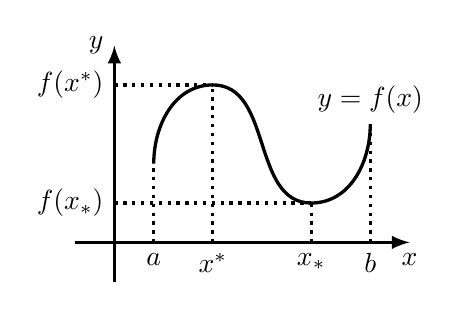
\begin{tikzpicture}[>=latex, very thick, scale = 0.5]
    %\draw [help lines, thin] (-3, -2) grid (7, 6);
    \draw [->] (-1, 0) -- (7.5, 0) node[below] {$x$};
    \draw [->] (0, -1) -- (0, 5) node[left]{$y$};
    %\draw (1, 2) .. controls (2, 6) and (4, -2) .. (5, 3);
    \draw[very thick] (1,2) to [out=90,in=180] (2.5, 4) to
    [out=0,in=180] (5,1) to [out=0,in=-90] (6.5,3);
    \draw[dotted] (0, 1) node[left]{$f(x_*)$} -- (5,1);
    \draw[dotted] (0, 4) node[left]{$f(x^*)$} -- (2.5,4);
    \draw[dotted] (2.5, 0) node[below]{$x^*$} -- (2.5,4);
    \draw[dotted] (1, 0) node[below]{$a$} -- (1, 2);
    \draw[dotted] (5, 0) node[below]{$x_*$} -- (5,1);
    \draw[dotted] (6.5, 0) node[below]{$b$} -- (6.5, 3) node[above]{$y = f(x)$};
    \end{tikzpicture}
  \caption{Теорема №21}
  \end{subfigure}
  \begin{subfigure}{0.3\textwidth}
    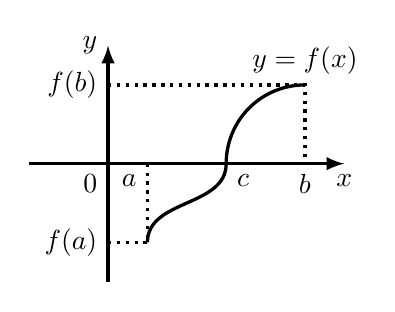
\begin{tikzpicture}[>=latex, very thick, scale = 0.5]
    %\draw [help lines, thin] (-4, -3) grid (7, 6);
    \draw [->] (-2, 0) -- (6, 0) node[below] {$x$};
    \draw [->] (0, -3) -- (0, 3) node[left]{$y$};
    \draw (0, 0) node [below left] {$0$};
    \draw[very thick] (1, -2) to [out=90, in=-90] (3,0) node[below right]{$c$} to [out=90, in=180] (5, 2);
    \draw[dotted] (1, 0) node[below left] {$a$} -- (1, -2);
    \draw[dotted] (0, -2) node[left] {$f(a)$} -- (1, -2);
    \draw[dotted] (0, 2) node[left] {$f(b)$} -- (5, 2) node[above]{$y=f(x)$} -- (5,0) node[below]{$b$};
    \end{tikzpicture}
  \caption{Теорема №22}
  \end{subfigure}
  \begin{subfigure}{0.3\textwidth}
    \begin{tikzpicture}[>=latex, very thick, scale = 0.5]
    %\draw[help lines, thin] (-0.5, -2) grid (8, 6);
    \draw (0,0) node[below left] {$0$};
    \draw[->] (-0.5, 0) -- (7, 0) node[below right] {$x$};
    \draw[->] (0, -1) -- (0, 4.5) node[left] {$y$};
    \draw [name path=graphic] (1, 1) to [out=90, in=180] (3, 3.6) to [out=0, in=170] (4, 3.3) to [out=0, in=210] (5, 3.5);
    \draw[dotted] (5, 3.5) -- (5, 0) node[below]{$b$};
    \draw[dotted] (5, 3.5) node[above]{$y = f(x)$} -- (0, 3.5) node[left]{$B = f(b)$};
    \draw[dotted] (1.5, 0) node[below]{$c$} |- (0, 2.75) node[left]{$C$};
    \draw[dotted] (1,0) node[below]{$a$} |- (0, 1) node[left]{$A=f(a)$};
    \end{tikzpicture}
  \caption{Теорема №23}
  \end{subfigure}
\end{figure}
  
\begin{theorem}[о существовании нуля непрерывной функции (\textbf{Первая теорема Больцана-Коши})]
  Если функция $y = f(x)$ непрерывна на отрезке $[a, b]$ и на концах отрезка принимает значения разных знаков, то $\exists\ c \in (a, b)\colon f(x) = 0$\\
  Кратко: \vspace{-\topsep}
  \begin{gather*}
    \big(f(x) \in C[a, b]\big) \wedge \big(f(x) \cdot f(b)< 0\big)\ \Rightarrow\ \big(\exists\ c \in (a, b)\big)\colon f(x) = 0
  \end{gather*}
\end{theorem}
  \begin{theorem}[о промежуточном значении непрерывной функции (\textbf{Вторая теорема Больцана-Коши})]
  Если функция $y = f(x)$ непрерывна на $[a, b]$ и принимает на границах отрезка различные значения ($f(a) = A \ne f(b) = B$), то $\forall C$, лежащего между $A$ и $B$, $\exists\ c \in (a, b),\ f(c) = C$\\
  Кратко: \vspace{-\topsep}
  \begin{gather*}
    \big(f(x) \in c[a, b]\big) \wedge \big(f(a) = A \ne f(b) = B\big)\ \Rightarrow\ \big(\forall\ C \in (A, B)\ \exists\ c \in (a, b)\ f(x) = C\big)
  \end{gather*}
\end{theorem}
\begin{theorem}[о существовании обратной к непрерывной функции]
  Пусть $y = f(x)$ непрерывна на интервале $(a, b)$ и строго монотонна (возрастает/убывает) на этом интервале. Тогда в соответствующем $(a, b)$ интервале значений функции существует обратная функция \big(обозначается $x = f^{-1}(y)$\big), которая также строго монотонна и непрерывна.
\end{theorem}
\newpage
\section{Сформулируйте определение точки разрыва функции и дайте классификацию точек разрыва. На каждый случай приведите примеры.}

\begin{definition}
  Пусть функция $y = f(x)$ определена в некоторой проколотой окрестности точки $x_0$, непрерывна в любой точке этой окрестности за исключением самой точки $x_0$.
  Тогда точка $x_0$ называется \textbf{точкой разрыва функции} $y = f(x)$.
\end{definition}
\begin{figure}[h]
  \begin{tikzcd}[row sep=10pt, column sep=-25pt, scale cd = 0.85]
    & & \arrow{dl} x_0 \text{ -- точка разрыва} \arrow{dr} & & \\
    & \arrow{dl} \begin{gathered} \text{I-го рода}\\ \exists \text{ конечные } \lim\limits_{x \to x_0 \pm} f(x) \end{gathered} \arrow{drr} & & \begin{gathered} \text{II-го рода}\\ \nexists \lim\limits_{x \to x_0\pm} f(x) \text{ или } \infty \end{gathered} & \\
    \begin{gathered} \text{точка конечного разрыва /}\\ \text{точка скачка}\\ \lim\limits_{x \to x_o +} f(x) \ne \lim\limits_{x\to x_0-} f(x) \\ \Delta f = \left|\lim\limits_{x \to x_o +} f(x) - \lim\limits_{x\to x_0-} f(x)\right| \end{gathered} & & & \begin{aligned} \text{точка устранимого разрыва}\\ \lim\limits_{x \to x_0+} f(x) = \lim\limits_{x \to x_0-} f(x) \ne f(x_0) \text{ или } \nexists f(x_0) \end{aligned} & \\
  \end{tikzcd}
\end{figure}
\vspace{-\topsep}
\begin{definition}
  Если точка $x_0$ --- точка разрыва функции $y = f(x)$ и существуют конечные пределы $\lim\limits_{x \to x_0+} f(x)$ и $\lim\limits_{x \to x_0-} f(x)$, то $x_0$ называют \textbf{точкой I-го рода}.
\end{definition}

\begin{definition}
  Если точка $x_0$ --- точка разрыва функции $y = f(x)$ и не существуют конечные пределы $\lim\limits_{x \to x_0+} f(x)$ и $\lim\limits_{x \to x_0-} f(x)$ или $\lim\limits_{x \to x_0} f(x) = \infty$, то $x_0$ называется \textbf{точкой разрыва II-го рода}.
\end{definition}

\begin{definition}
  Если точка $x_0$ --- точка разрыва первого рода функции $y = f(x)$ и предел $\lim\limits_{x \to x_0+} f(x) \neq \lim\limits_{x \to x_0-} f(x)$, то $x_0$ называется \textbf{точкой конечного разрыва} или точкой \textit{скачка}.
\end{definition}

\begin{definition}
  Если точка $x_0$ --- точка разрыва первого рода функции $y = f(x)$ и предел  $\lim\limits_{x \to x_0+} f(x) = \lim\limits_{x \to x_0-} f(x)$, но $\nexists f(x_0)$, то точка $x_0$ называется \textbf{точкой устранимого разрыва}.
\end{definition}
\newpage
\subsubsection*{Примеры}

\begin{eg}
  $\displaystyle y = \frac{|x - 1|}{x - 1}\qquad D_f = \R \setminus \{1\}\qquad x = 1 \text{ --- точка разрыва}$ \\
  \begin{gather*}
    \begin{aligned}
      \lim_{x \to 1+} f(x) &= \lim_{x \to 1+} \frac{|x - 1|}{x - 1} = \frac{x - 1}{x - 1} = 1 \\
      \lim_{x \to 1-} f(x) &= \lim_{x \to 1-} \frac{|x - 1|}{x - 1} = \frac{1 - x}{x - 1} = -1
    \end{aligned}\ \Rightarrow\ \lim_{x \to 1+} f(x) \neq \lim_{x \to 1-} f(x)\ \Rightarrow \\[1ex]
  \Rightarrow\ x = 1 \text{ --- т.р. I рода, точка скачка}\\
  \Delta f = \left|\lim_{x \to 1+} f(x) - \lim_{x \to 1-} f(x)\right| = \big|1 - (-1)\big| = 2  
  \end{gather*}
\end{eg}

\begin{eg}
  $\displaystyle y = \frac{\sin x}{x}\qquad D_f = \R \setminus \{0\}\qquad x=0 \text{ --- точка разрыва}$ \\
  \begin{gather*}
    \begin{aligned}
      \lim_{x \to 0+} f(x) &= \lim_{x \to 0+} \frac{\sin x}{x} = 1 \\
      \lim_{x \to 0-} f(x) &= \lim_{x \to 0-} \frac{\sin x}{x} = 1 \\
    \end{aligned}\ \Rightarrow\ \lim_{x \to 0+} f(x) = \lim_{x \to 0-} f(x)\ \Rightarrow \\[1ex]
    \Rightarrow\ x = 0 \text{ --- т.р. I рода, устранимая точка разрыва} \\[1ex]
    g(x) = \begin{cases}
      \dfrac{\sin x}{x}, x \neq 0 \\
      1, x = 0
    \end{cases} \\[1ex]
    f(x) \notin C(0) \\
    g(x) \in C(0)
  \end{gather*}
\end{eg}
\begin{eg}
  $y = e^{\tfrac{1}{x}}\qquad D_f = \R \setminus \{0\}\qquad x=0 \text{ --- точка разрыва}$ \\
  \begin{gather*}
    \begin{aligned}
      \lim_{x \to 0+} f(x) &= \lim_{x \to 0+} e^{\tfrac{1}{x}} = e^{+\infty} = \infty \\ 
      \lim_{x \to 0-} f(x) &= \lim_{x \to 0-} e^{\tfrac{1}{x}} = e^{-\infty} = 0 \\ 
    \end{aligned}\ \Rightarrow\ \lim_{x \to 0+} f(x) = \infty\ \Rightarrow\ x = 0 \text{ --- т.р. II рода}
  \end{gather*}
\end{eg}

\newpage
\section{Сформулируйте и докажите необходимое и достаточное условие существования наклонной асимптоты.}

\begin{theorem}[Необходимое и достаточное условие существования наклонных асимптот]
	График функции $y=f(x)$ имеет при $x\to \pm \infty$ наклонную асимптоту тогда и только тогда, когда существуют два конечных передела:
	\begin{gather*}
		\left\{ \begin{aligned}
			 & \lim\limits_{x \to \pm \infty} \frac{f(x)}{x} = k               \\
			 & \lim\limits_{x \to \pm \infty} \big(f(x) - k\cdot x\big) = b
		\end{aligned} \tag{$*$} \right.
	\end{gather*}
\end{theorem}
\begin{proof}[][Необходимость]
	\textbf{Дано}: $y=kx+b$ --- наклонная асимптота\\
	\textbf{Доказать}: $\exists$ конечные пределы $(*)$\\
	По условию $kx+b$ наклонная асимптота $\Rightarrow$ по определению наклонной асимптоты (\textbf{опр.\ref{опр: наклонная асимптота}}): $f(x) = kx + b + \alpha(x)$, где $\alpha(x)$ -- б.м.ф. при $x \to \pm \infty$.\\
	Рассмотрим:
	\begin{flalign*}
		\lim\limits_{x \to \pm \infty} \frac{f(x)}{x} = \lim\limits_{x \to \pm \infty} \frac{kx + b + \alpha(x)}{x} & = \lim\limits_{x \to \pm \infty} \left(k + b\cdot \frac{1}{x} + \frac{1}{x}\cdot \alpha(x)\right) = & \\
    & = k + b\cdot \lim\limits_{x \to \pm \infty} \frac{1}{x} + \lim\limits_{x  \to \pm \infty} \frac{1}{x}\cdot \alpha(x) = k + b\cdot 0 + 0 = k &
	\end{flalign*}
	Рассмотрим выражение:
	\begin{gather*}
		f(x) - k\cdot x = \cancel{kx} + b + \alpha(x) - \cancel{kx} = b + \alpha(x)
	\end{gather*}
	Вычислим:
	\begin{flalign*}
		 & \lim\limits_{x \to \pm \infty} \big(f(x) - k\cdot x\big) = \lim\limits_{x \to \pm \infty} \big(b + \alpha(x)\big) = b + \lim\limits_{x \to \pm \infty} \alpha(x) = b + 0 = b
	\end{flalign*}
\end{proof}
\begin{proof}[][Достаточность]
	\textbf{Дано}: $\exists$ конечные пределы $(*)$\\
	\textbf{Доказать}: $y=kx+b$ --- наклонная асимптота\\[1ex]
	$\exists$ конечный предел: $\lim\limits_{x \to \pm \infty} (f(x) - kx) = b$\\
	По теореме \textit{о связи функции, её предела и б.м.ф.} (\textbf{Т.\ref{О связи функции, её предела и б.м.ф.}}) $\Rightarrow$\\
	$\Rightarrow\ f(x) - kx = b + \alpha(x)$, где $\alpha(x)$ -- б.м.ф. при $x \to \pm \infty$.\\
	Выразим $f(x) = kx + b + \alpha(x)$, где $\alpha(x)$ -- б.м.ф. при $x \to \pm \infty$.\\
	По определению наклонной асимптоты $\Rightarrow\ y = kx + b$ --- наклонная асимптота графика функции $y=f(x)$.
\end{proof}

\newpage
\section{Сформулируйте и докажите необходимое и достаточное условие дифференцируемости функции в точке.}

\begin{theorem}[Необходимое и достаточное условие дифференцируемости функции]\hlabel{Условие дифференцируемости}
  Функция $y=f(x)$ дифференцируема в точке $x_0$ тогда и только тогда, когда она имеет в этой точке конечную производную.
\end{theorem}
\begin{proof}[][Необходимость]
  \textbf{Дано}: $y=f(x)$ дифференцируема в точке $x_0$\\
  \textbf{Доказать}: $\exists\ y'(x_0)$ -- конечное число\\
  Т.к. $y=f(x)$ дифференцируема в точке $x_0$, то $\Delta y = A\cdot \Delta x + \alpha(\Delta x) \cdot \Delta x$, \\ где $\alpha (\Delta x)$ -- б.м.ф. при $\Delta x \to 0$\\
  Вычислим предел:
  \begin{flalign*}
  & \lim\limits_{\Delta x \to 0} \frac{\Delta y}{\Delta x} = \lim\limits_{\Delta x \to 0} \frac{A\cdot \Delta x + \alpha(\Delta x) \cdot \Delta x}{\Delta x} = \lim\limits_{\Delta x \to 0} (A + \alpha (\Delta x)) = A  + \lim\limits_{\Delta x \to 0} \alpha(\Delta x) = &\\
  & = A + 0 = A &\\
  & \lim\limits_{\Delta x \to 0} \frac{\Delta x}{\Delta y} = y'(x_0) \text{ -- по определению производной в точке } (\textbf{опр.\ref{опр: производная функции}}) &\\
  & y'(x_0) = A = const\ \Rightarrow\ \exists\ y'(x_0) \text{ -- конечное число} & 
  \end{flalign*} 
\end{proof}
\begin{proof}[][Достаточность]
  \textbf{Дано}: $\exists\ y'(x_0)$ -- конечное число\\
  \textbf{Доказать}: $y=f(x)$ дифференцируема в точке $x_0$\\
  Т.к. $\exists\ y'(x_0)$, то по определению производной: $y'(x_0) = \lim\limits_{\Delta x \to 0} \dfrac{\Delta y}{\Delta x}$\\\\
  По теореме \textit{о связи функции, её предела и б.м.ф.} (\textbf{c.\pageref{О связи функции, её предела и б.м.ф.}, Т.\ref{О связи функции, её предела и б.м.ф.}}) $\Rightarrow\ \dfrac{\Delta y}{\Delta x} = y'(x_0) + \alpha (\Delta x)$,\\\\ где $\alpha (\Delta x)$ -- б.м.ф. при $\Delta x \to 0$ \\
  $\Delta y = y'(x_0)\cdot \Delta x + \alpha (\Delta x) \cdot \Delta x$, где $\underbrace{y'(x_0)}_{A}$ -- $const\ \Rightarrow$\\
  $\Rightarrow\ y=f(x)$ дифференцируема в точке $x_0$
\end{proof}
\begin{corollary}
  Функция, выражающая дифференцируемость функции $y=f(x)$ в точке $x_0$ примет вид:
  \[ \boxed{\Delta y = y'(x_0)\cdot \Delta x + \alpha (\Delta x) \cdot \Delta x} \]
  где $\alpha (\Delta x)$ -- б.м.ф. при $\Delta x \to 0$
\end{corollary}

\newpage
\section{Сформулируйте и докажите теорему о связи дифференцируемости и непрерывности функции.}

\begin{theorem}[Связь дифференцируемости и непрерывности функции] \hlabel{Связь диф. и непр. функции}
  Если функция дифференцируема в точке $x_0$, то она в этой точке непрерывна.
\end{theorem}
\begin{proof}
  Т.к. $y=f(x)$ дифференцируема в точке $x_0$, то $\Delta y = y'(x_0)\cdot \Delta x + \alpha (\Delta x) \cdot \Delta x$, где $y'(x_0) = const$,\quad $\alpha (\Delta x)$ -- б.м.ф. при $\Delta x \to 0$\\
  Вычислим:
  \begin{align*}
  \lim\limits_{\Delta x \to 0} \Delta y &= \lim\limits_{\Delta x \to 0} \big(y'(x_0)\cdot \Delta x + \alpha (\Delta x) \cdot \Delta x\big) = \\
  &= y'(x_0)\cdot \lim\limits_{\Delta x \to 0} \Delta x + \lim\limits_{\Delta x \to 0} \alpha(\Delta x)\cdot \lim\limits_{\Delta x \to 0} \Delta x = y'(x_0) \cdot 0 + 0\cdot 0 = 0
  \end{align*}
  По определению непрерывной функции (\textbf{опр.\ref{опр: функция непрерывная в точке}}) $y=f(x)$ непрерывна в точке $x_0$.
\end{proof}
\begin{center}
  \fbox{\pbox[c][20pt]{5cm}{дифференцируемость}} $\begin{aligned} \Longrightarrow\\ \cancel{\Longleftarrow} \end{aligned}$ \fbox{\pbox[c][20pt]{5cm}{непрерывность}}
\end{center}
\begin{eg}
  $y = |x|,\ x_0 = 0$ является непрерывной, но не является дифференцируемой
\end{eg}

\section{Сформулируйте и докажите теорему о производной произведения двух дифференцируемых функций.}

\begin{theorem}[Производная произдведения]
  Пусть функции $u = u(x),\ \upsilon = \upsilon (x)$ дифференцируемы в точке $x$.\\
  Тогда в этой точке дифференцируемо их произведение и справедливо равенство:
    \[ (u \cdot \upsilon)' = u'\cdot \upsilon + \upsilon' \cdot u \]
\end{theorem}
\vspace{-11pt}
\begin{mdframed}[
linecolor= RosyBrown!50!black,
linewidth = 2pt,
backgroundcolor = RosyBrown!8!white,
innertopmargin = 5pt,
topline = false, 
bottomline = false, 
rightline = false,
skipabove = 1pt,
skipbelow = 20pt,
]
  Распишем приращения каждой из функций:
  \begin{flalign*}
    & \left\{ \begin{aligned}
    \Delta u = u(x + \Delta x) - u(x)\\
    \Delta \upsilon = \upsilon (x + \Delta x) - \upsilon (x)
    \end{aligned}  \right. \Rightarrow\ \left\{ \begin{aligned}
    u(x + \Delta x) = \Delta u + u(x)\\
    \upsilon (x + \Delta x) = \Delta \upsilon + \upsilon (x)
    \end{aligned} \right. &
  \end{flalign*}
\end{mdframed}
\begin{proof}[][Производная произведения]
  Пусть $y=u\cdot \upsilon$, тогда: \vspace{-\topsep}
  \begin{flalign*}
    \Delta y &= y(x + \Delta x) - y(x) = u(x + \Delta x)\cdot \upsilon (x+\Delta x) - u(x)\cdot \upsilon(x) = &\\
    & = \big(\Delta u + u(x)\big)\cdot\big(\Delta \upsilon + \upsilon(x)\big) - u(x)\cdot \upsilon(x) = &\\
    & = \Delta u \cdot \Delta \upsilon + \Delta u \cdot \upsilon(x) + \Delta \upsilon \cdot u(x) + \cancel{u(x) \cdot \upsilon (x)} - \cancel{u(x) \cdot \upsilon (x)} = &\\
    & = \Delta u \cdot \Delta \upsilon + \Delta u \cdot \upsilon (x) + \Delta \upsilon \cdot u(x) &
  \end{flalign*}
  Вычислим: 
  \begin{flalign*}
    y'(x) &= \lim_{\Delta x \to 0} \frac{\Delta y}{\Delta x} = \lim_{\Delta x \to 0} \frac{\Delta u \cdot \Delta \upsilon + \Delta u \cdot \upsilon(x) + \Delta \upsilon \cdot u(x)}{\Delta x} = &\\
    & = \lim_{\Delta x \to 0} \left( \Delta u \frac{\Delta \upsilon}{\Delta x} + \upsilon(x) \frac{\Delta u}{\Delta x} + u(x)\frac{\Delta \upsilon}{\Delta x} \right) = &\\
    & = \lim_{\Delta x \to 0} \Delta u \cdot \lim_{\Delta x \to 0} \frac{\Delta \upsilon}{\Delta x} + \upsilon(x) \cdot \lim_{\Delta x \to 0} \frac{\Delta u}{\Delta x} + u(x) \cdot \lim_{\Delta x \to 0} \frac{\Delta \upsilon}{\Delta x} = &\\ 
    & = 0 \cdot \upsilon'(x) + \upsilon (x) \cdot u'(x) + u(x)\cdot \upsilon'(x) = \boxed{\upsilon(x) \cdot u'(x) + u(x) \cdot \upsilon'(x)} &
  \end{flalign*}
  Т.к. функции $u=u(x),\ \upsilon = \upsilon(x)$ дифференцируемы в точке $x$, то по теореме \textit{о связи дифференцируемости и непрерывности функции} (\textbf{Т.\ref{Связь диф. и непр. функции}}) $\Rightarrow\ u=u(x)$ и $\upsilon = \upsilon(x)$ непрерывны в точке $x\ \Rightarrow$ по определению \stackunder{непрерывной}{\footnotesize{(\textbf{опр.\ref{опр: функция непрерывная в точке}})}} функции: $\left\{ \begin{aligned}
  \lim\limits_{\Delta x \to 0} \Delta u = 0\\
  \lim\limits_{\Delta x \to 0} \Delta \upsilon = 0
  \end{aligned} \right.$
\end{proof}

\section{Сформулируйте и докажите теорему о производной частного двух дифференцируемых функций.}

\begin{theorem}[Производная частного]
  Пусть функции $u = u(x),\ \upsilon = \upsilon (x)$ дифференцируемы в точке $x$.\\
  Тогда в этой точке дифференцируемо их частное (при условии $\upsilon \ne 0$) и справедливо равенство:
    \[ \left(\dfrac{u}{\upsilon}\right)' = \dfrac{u' \cdot \upsilon - \upsilon' \cdot u}{\upsilon^2} \]
\end{theorem}
\vspace{-11pt}
\begin{mdframed}[
linecolor= RosyBrown!50!black,
linewidth = 2pt,
backgroundcolor = RosyBrown!8!white,
innertopmargin = 5pt,
topline = false, 
bottomline = false, 
rightline = false,
skipabove = 1pt,
skipbelow = 20pt,
]
  Распишем приращения каждой из функций:
  \begin{flalign*}
    & \left\{ \begin{aligned}
    \Delta u = u(x + \Delta x) - u(x)\\
    \Delta \upsilon = \upsilon (x + \Delta x) - \upsilon (x)
    \end{aligned}  \right. \Rightarrow\ \left\{ \begin{aligned}
    u(x + \Delta x) = \Delta u + u(x)\\
    \upsilon (x + \Delta x) = \Delta \upsilon + \upsilon (x)
    \end{aligned} \right. &
  \end{flalign*}
\end{mdframed}
\begin{proof}[][Производная частного]
  Пусть $y = \dfrac{u}{\upsilon}$, тогда: \vspace{-\topsep}
  \begin{flalign*}
    \Delta	y &= y(x+ \Delta x) - y(x) = \frac{u(x + \Delta x)}{\upsilon (x + \Delta x)} - \frac{u(x)}{\upsilon(x)} = \frac{u(x+\Delta x)\cdot \upsilon(x) - u(x) \cdot \upsilon (x + \Delta x)}{\upsilon(x+ \Delta x)\cdot \upsilon (x)} = &\\
    & = \begin{vmatrix}
    u(x+\Delta x) = u(x) + \Delta u \\
    \upsilon(x + \Delta x) = \upsilon (x) + \Delta \upsilon
    \end{vmatrix} = \frac{(u(x) + \Delta u) \cdot \upsilon (x) - u(x) \cdot (\upsilon(x) + \Delta \upsilon)}{(\Delta \upsilon + \upsilon(x)) \cdot \upsilon(x)} = &\\
    & = \frac{\cancel{u(x)\cdot \upsilon(x)} + \Delta u \cdot \upsilon (x) - \cancel{u(x)\cdot \upsilon(x)} - u(x) \cdot \Delta \upsilon}{\upsilon^2 (x) + \upsilon(x) \cdot \Delta \upsilon} = \frac{\Delta u \cdot \upsilon (x) - \Delta \upsilon \cdot u(x)}{\upsilon^2(x) + \upsilon(x) \cdot \Delta \upsilon} &
  \end{flalign*} 
  Вычислим предел: \vspace{-\topsep}
  \begin{flalign*}
    y'(x) &= \lim_{\Delta x \to 0} \frac{\Delta y}{\Delta x} = \lim_{\Delta x \to 0} \frac{\displaystyle \frac{\Delta u \cdot \upsilon (x) - \Delta \upsilon \cdot u(x)}{\upsilon^2(x) + \upsilon(x) \cdot \Delta \upsilon}}{\Delta x} = \lim_{\Delta x \to 0} \frac{\upsilon(x) \dfrac{\Delta u}{\Delta x} - u(x) \dfrac{\Delta \upsilon}{\Delta x}}{\upsilon^2(x) + \upsilon(x)\cdot \Delta \upsilon} = &\\
    & = \frac{\upsilon(x) \cdot \lim\limits_{\Delta x \to 0}\dfrac{\Delta u}{\Delta x} - u(x) \cdot \lim\limits_{\Delta x \to 0} \dfrac{\Delta \upsilon}{\Delta x}}{\upsilon^2(x) - \upsilon (x) \lim\limits_{\Delta x \to 0}\Delta \upsilon} = \frac{\upsilon(x) \cdot u'(x) - u(x) \cdot \upsilon'(x)}{\upsilon^2(x) + \upsilon(x) \cdot 0} = &\\
    & = \boxed{\frac{\upsilon(x)\cdot u'(x) - u(x)\cdot \upsilon'(x)}{\upsilon^2(x)}} &
  \end{flalign*}
  Использовали: $\lim\limits_{\Delta x \to 0} \dfrac{\Delta u}{\Delta x} = u'(x)\qquad \lim\limits_{\Delta x \to 0} \dfrac{\Delta \upsilon}{\Delta x} = \upsilon'(x)$\\
  Так как $\upsilon(x)$ -- дифференцируема, то по теореме \textit{о связи дифференцируемости и непрерывности функции} (\textbf{Т.\ref{Связь диф. и непр. функции}}) $\upsilon(x)$ -- непрерывна $\Rightarrow$ по определению непрерывности (\textbf{опр.\ref{опр: функция непрерывная в точке}}) $\lim\limits_{\Delta x \to 0} \Delta \upsilon = 0$. \vspace{-\topsep}
  \[ \left(\frac{u}{\upsilon}\right)' = \frac{u'\cdot \upsilon - \upsilon' \cdot u}{\upsilon^2}  \]
\end{proof}

\section{Сформулируйте и докажите теорему о производной сложной функции.}

\begin{theorem}[Производная сложной функции]\hlabel{Производная сложной функции}
  Пусть функция $u=g(x)$ дифференцируема в точке $x=a$, а функция $y=f(u)$ дифференцируема в соответствующей точке $b=g(a)$. \\
  Тогда сложная функция $F(x) = f(g(x))$ дифференцируема в точке $x=a$ и \[ F'(x) \Big|_{x=a} = \Big(f\big(g(x)\big)\Big)' \Big|_{x=a} = f'_u(b)\cdot g'_x(a) \]
\end{theorem}
\begin{proof}
  Так как функция $u=g(x)$ дифференцируема в точке $x=a$, то по определению дифференцируемости (\textbf{опр.\ref{опр: дифференцируемая функция}}):\vspace{-\topsep}
  \begin{align}
    \boxed{\Delta u = g'(a)\cdot \Delta x + \alpha(\Delta x) \cdot \Delta x }
  \end{align}
  где $\alpha (\Delta x)$ -- б.м.ф. при $\Delta x \to 0$\\
  Так как функция $y=f(u)$ дифференцируема в точке $b$, то по определению дифференцируемости: \vspace{-\topsep}
  \begin{align}
    \boxed{\Delta y = f'(b)\cdot \Delta u + \beta (\Delta u) \cdot \Delta u }
  \end{align}
  где $\beta (\Delta u)$ -- б.м.ф. при $\Delta u \to 0$\\
  Подставим (1) в (2): 
  \begin{flalign*}
    \Delta y &= f'(b) \cdot \Big(g'(a)\cdot \Delta x + \alpha(\Delta x) \cdot \Delta x\Big) + \beta(\Delta u) \cdot \Big(g'(a)\cdot \Delta x + \alpha (\Delta x) \cdot \Delta x\Big) =  &\\
    & = f'(b) \cdot g'(a) \cdot \Delta x + \Delta x \cdot \Big(f'(b) \cdot \alpha (\Delta x) + g'(a) \cdot \beta (\Delta u) + \beta (\Delta u) \cdot \alpha (\Delta x)\Big)' = \Delta F &
  \end{flalign*} 
  Обозначим: \[ \gamma (\Delta x) = f'(b)\cdot \alpha (\Delta x) + g'(a) \cdot \beta (\Delta u) + \beta (\Delta u) \cdot \alpha (\Delta x) \]
  В итоге получаем: \[ \Delta F = f'(b) \cdot g'(a) \cdot \Delta x + \gamma ( \Delta x) \cdot \Delta x \]
  $f'(b)\cdot \alpha(\Delta x)$ -- б.м.ф. при $\Delta x \to 0$ (как произведение постоянной на б.м.ф)\\
  Так как $u=g(x)$ дифференцируема в точке $x=a$, то по теореме \textit{о связи дифференцируемости и непрерывности функции} (\textbf{Т.\ref{Связь диф. и непр. функции}}) $\Rightarrow\ u=g(x)$ непрерывна в точке $x=a\ \Rightarrow$\\
  $\Rightarrow$ по определению непрерывности (\textbf{опр.\ref{опр: функция непрерывная в точке (приращение)}}) $\lim\limits_{\Delta x \to 0} \Delta u = 0$ или при $\Delta x \to 0,\ \Delta u \to 0$ \vspace{-\topsep}
  \begin{align*}
    &\left. \begin{aligned}
    g'(a)\cdot \beta(\Delta u) &\text{ -- б.м.ф. при } \Delta x \to 0 \text{ (как произведение постоянной на б.м.ф.)}\\
    \beta (\Delta u) \cdot \alpha (\Delta x) &\text{ -- б.м.ф. при } \Delta x \to 0 \text{ (как произведение двух б.м.ф.)}
    \end{aligned}\right| \Rightarrow \\
    &\hspace{23pt} \Rightarrow\ \gamma(\Delta x) \text{ -- б.м.ф. при } \Delta x \to 0 \text{ (как сумма конечного числа б.м.ф.)} 
  \end{align*} 
  Вычислим предел:
  \begin{flalign*}
    & \lim_{\Delta x \to 0} \frac{\Delta F}{\Delta x} = \lim_{\Delta x \to 0} \Big(f'(b)\cdot g'(a) + \gamma(\Delta x)\Big) = f'(b)\cdot g'(a) + 0 = f'(b)\cdot g'(a) &
  \end{flalign*}
\end{proof}

\section{Сформулируйте и докажите теорему о производной обратной функции.}

\begin{theorem}[Производная обратной функции]
  Пусть функция $y=f(x)$ в точке $x=a$ имеет конечную и отличную от нуля производную $f'(a)$ и пусть для неё существует однозначная обратная функция $x = g(y)$, непрерывная в соответствующей точке $b=f(a)$. Тогда существует производная обратной функции и она равна \[ g'(b) = \frac{1}{f'(a)} \]
\end{theorem}
\begin{proof}
  Так как функция $x = g(y)$ однозначно определена $\Rightarrow$ при $\Delta y \ne 0,\ \Delta x \ne 0$\\
  Так как функция $x=g(y)$ непрерывна в точке $b \Rightarrow \lim\limits_{\Delta y \to 0} \Delta x = 0$ или $\Delta x \to 0$ при $\Delta y \to 0$
  \begin{flalign*}
    & g'(b) = \lim_{\Delta y \to 0} \frac{\Delta x}{\Delta y} = \lim_{\Delta y \to 0}\frac{1}{\frac{\Delta y }{\Delta x}} = \frac{1}{\lim\limits_{\Delta y \to 0} \dfrac{\Delta y}{\Delta x}} = \frac{1}{\lim\limits_{\Delta x \to 0} \dfrac{\Delta y}{\Delta x}} = \frac{1}{f'(a)} &
  \end{flalign*}
\end{proof}

\newpage
\section{Сформулируйте и докажите свойство инвариантности формы записи дифференциала первого порядка.}

Формула первого дифференциала: \vspace{-\topsep}
\begin{gather*}
  \boxed{dy = f'(x)dx} \tag{1}
\end{gather*} 
$x$ -- неизвестная переменная\\
Докажем, что формула (1) верна и в том случае, когда $x$ -- функция другой переменной.\\ \setcounter{equation}{0}
\begin{theorem}[Инвариантность формы первого дифференциала]
  Форма записи первого дифференциала не зависит от того, является ли $x$ независимой переменной или функцией другого аргумента.
\end{theorem}
\begin{proof}
  Пусть $\begin{aligned}
    &y=f(x)\\
    &x=\varphi (t)
  \end{aligned}$, тогда можно задать сложную функцию $F(t) = y = f(\varphi (t))$\\
  По определению дифференциала функции (\textbf{опр.\ref{опр: дифференциал}}):
  \begin{gather}
    dy = F'(t)dt
  \end{gather} 
  По теореме \textit{о производной сложной функции} (\textbf{Т.\ref{Производная сложной функции}}):
  \begin{gather}
    F'(t) = f'(x) \cdot \varphi'(t)
  \end{gather} 
  Подставим (2) в (1): \vspace{-\topsep}
  \begin{gather}
    dy = f'(x) \cdot \varphi'(t)dt
  \end{gather}
  По определению дифференцируемой функции (\textbf{опр.\ref{опр: дифференцируемая функция}}):
  \begin{gather}
    dx = \varphi'(t)dt
  \end{gather}
  Подставим (4) в (3): \vspace{-1.5\topsep}
  \begin{gather*}
    \boxed{dy = f'(x)dx}
  \end{gather*} 
\end{proof}
\setcounter{equation}{0}
\begin{corollary}
  Свойством инвариантности обладает только первый дифференциал. 
\end{corollary} 

\section{Сформулируйте и докажите теорему Ферма.}

\begin{theorem}[\textbf{Теорема Ферма} (о нулях производной)]\hlabel{Ферма}
	Пусть функция $y=f(x)$ определена на промежутке $X$ и во внутренней точке $\bm{c}$ этого промежутка достигает наибольшего или наименьшего значения. Если в этой точке существует производная $f'(c)$, то $f'(c) = 0$.
\end{theorem}
\begin{proof}
	Пусть функция $y=f(x)$ в точке $x=c$ принимает наибольшее значение на промежутке $X\Rightarrow\ \forall x \in X\ \Rightarrow\ f(x)\le f(c)$\\
	Дадим приращение $\Delta x$ в точке $x=c$, тогда $f(c + \Delta x) \le f(c)$.\\[1ex]
	Пусть $\exists\ f'(c) = \lim\limits_{\Delta x \to 0}\dfrac{\Delta y}{\Delta x} = \lim\limits_{\Delta x \to 0}\dfrac{y(c+ \Delta x) - y(c)}{\Delta x}$\\[1ex]
	Рассмотрим два случая:
	\begin{enumerate}
		\item $\Delta x > 0,\ \Delta x \to 0+,\ x \to c+$
		      \begin{flalign*}
			       & f'_+(c) = \lim_{\Delta x \to 0+}\frac{y(c+ \Delta  x) - y(c)}{\Delta x} = \left( \frac{-}{+}\right) \le 0 &
		      \end{flalign*}
		\item $\Delta x < 0,\ \Delta x \to 0-,\ x \to c-$
		      \begin{flalign*}
			       & f'_-(c) = \lim_{\Delta x \to 0-}\frac{y(c+ \Delta  x) - y(c)}{\Delta x} = \left( \frac{-}{-}\right) \ge 0 &
		      \end{flalign*}
	\end{enumerate}
	По теореме \textit{о существовании производной функции в точке} (\textbf{Т.\ref{Существование производной функции в точке}}):
	\begin{gather*}
		f'(c) = f'_+(c) = f'_-(c) = 0
	\end{gather*}
\end{proof}

\section{Сформулируйте и докажите теорему Ролля.}

\begin{theorem}[\textbf{Теорема Ролля}]\hlabel{Ролль}
	Пусть $y=f(x)$
	\begin{enumerate}
		\item непрерывна на $[a;b]$
		\item дифференцируема на $(a;b)$
		\item $f(a) = f(b)$
	\end{enumerate}
	Тогда $\exists\ c \in (a;b)\colon f'(c) = 0$
\end{theorem}
\begin{proof}
	Так как функция $y=f(x)$ непрерывна на $[a;b]$, то по теореме \textit{Вейерштрасса} (\textbf{Т.\ref{Вейерштрасса 2}}) она достигает на этом отрезке своего наибольшего и наименьшего значений.\\
	Возможны два случая:
	\begin{enumerate}
		\item Наибольшее и наименьшее значения достигаются на границе, то есть в точке $a$ и в точке $b$\\
		      $M=m$, где $\begin{aligned}
				       & m \text{ -- наименьшее} \\
				       & M \text{ -- наибольшее}
			      \end{aligned}\ \Rightarrow\ y=f(x)=const \text{ на } [a;b]\ \Rightarrow\\[1ex]
			      \Rightarrow\ \forall x \in (a;b)\colon f'(x)=0$
		\item Наибольшее или наименьшее значение достигается во внутренней точке $(a;b)$.\\
		      Тогда для функции $y=f(x)$ справедлива теорема \textit{Ферма} (\textbf{Т.\ref{Ферма}}) $\Rightarrow$\\
		      $\Rightarrow\ \exists\ c \in (a;b)\colon f'(c) = 0$
	\end{enumerate}
\end{proof}

\newpage
\section{Сформулируйте и докажите теорему Лагранжа.}

\begin{theorem}[\textbf{Теорема Лагранжа}]\hlabel{Лагранж}
	Пусть функция $y=f(x)$
	\begin{enumerate}
		\item непрерывна на $[a;b]$
		\item дифференцируема на $(a;b)$
	\end{enumerate}
	Тогда $\exists\ c \in (a;b)\colon \boxed{f(b) - f(a) = f'(c) \cdot (b-a)}$
\end{theorem}
\begin{proof}
	Рассмотрим вспомогательную функцию: $F(x) = f(x) - f(a) - \dfrac{f(b) - f(a)}{b - a} \cdot (x-a)$\\
	$F(x)$ непрерывна на $[a;b]$ как сумма непрерывных функций.\\
	Существует конечная производная функции $F(x)$. \vspace{-\topsep}
	\begin{flalign*}
    & F'(x) = f'(x) - \frac{f(b) - f(a)}{b-a} \Rightarrow\ \begin{aligned}  & \textit{необходимому и достаточному} \\
    & \textit{условию дифференцируемости }\end{aligned}\ (\textbf{Т.\ref{Условие дифференцируемости}}) \Rightarrow & \\
    & \Rightarrow\ F(x) \text{ --- дифференцируема на } (a;b)&
	\end{flalign*}
	Покажем, что $F(a) = F(b)$:
	\begin{flalign*}
    & F(a) = f(a) - f(a) - \frac{f(b) - f(a)}{b - a} \cdot(a - a) = 0 & \\
    & F(b) = f(b) - f(a) - \frac{f(b) - f(a)}{b - a} \cdot(b - a) = f(b) - f(a) - f(b) + f(a) = 0 &
	\end{flalign*}
	$\Rightarrow\ F(x)$ удовлетворяет условиям теоремы \textit{Ролля} (\textbf{Т.\ref{Ролль}}) \\
	По теореме \textit{Ролля} $\Rightarrow\ \exists\ c \in (a;b) \qquad F'(c) = 0$
	\begin{flalign*}
		 & F'(x) = f'(x) - \frac{f(b) - f(a)}{b - a}     & \\
		 & F'(c) = f'(c) - \frac{f(b) - f(a)}{b - a} = 0 & \\
		 & f'(c) = \frac{f(b) - f(a)}{b - a}             & \\
		 & f(b) - f(a) = f'(c) \cdot (b-a)
	\end{flalign*}
\end{proof}

\newpage
\section{Сформулируйте и докажите теорему Коши.}

\begin{theorem}[\textbf{Теорема Коши}]\label{Коши}
	Пусть функции $f(x)$ и $\varphi (x)$
	\begin{enumerate}
		\item непрерывны на $[a;b]$
		\item дифференцируемы на $(a;b)$
		\item $\forall x \in (a;b)\colon \varphi' (x) \ne 0$
	\end{enumerate}
	Тогда $\exists\ c \in (a;b)\colon$ \vspace{-\topsep}
	\begin{gather*}
		\boxed{\frac{f(b) - f(a)}{\varphi (b) - \varphi (a)} = \frac{f'(c)}{\varphi'(c)}}
	\end{gather*}
\end{theorem} 
\begin{proof}
	Рассмотрим вспомогательную функцию:
	\begin{gather*}
		F(x) = f(x) - f(a) - \frac{f(b) - f(a)}{\varphi(b) - \varphi(a)} \cdot \Big(\varphi(x) - \varphi(a)\Big)
	\end{gather*}
	\begin{enumerate}
		\item $F(x)$ непрерывна на $[a;b]$ как линейная комбинация непрерывных функций
		\item $F(x)$ дифференцируема на $(a;b)$ как линейная комбинация дифференцируемых функций
		\item $F(a) = F(b)$
	\end{enumerate}\vspace{-\topsep}
	\begin{flalign*}
		 & F(a) = \cancel{f(a)} - \cancel{f(a)} - \frac{f(b)-f(a)}{\varphi(b) - \varphi(a)}\cdot(\underbrace{\varphi(a) - \varphi(a)}_{0})=0                             & \\
		 & F(b) = f(b) - f(a) - \frac{f(b) - f(a)}{\cancel{\varphi(b) - \varphi(a)}}\cdot\Big(\cancel{\varphi(b)-\varphi(a)}\Big)= \cancel{f(b)}- \bcancel{f(a)} - \cancel{f(b)} + \bcancel{f(a)} = 0 &
	\end{flalign*}
	Функция $F(x)$ удовлетворяет условию теоремы \textit{Ролля} (\textbf{Т.\ref{Ролль}}).\\
	По теореме \textit{Ролля} $\Rightarrow$ $\exists\ c \in (a;b)\colon F'(c) = 0$\\[1ex]
	Вычислим $F'(x) = f'(x) -\dfrac{f(b)-f(a)}{\varphi(b) - \varphi(a)}\cdot \varphi'(x)$
	\begin{flalign*}
		 & F'(c) = f'(c) - \frac{f(b) - f(a)}{\varphi(b) - \varphi(a)} \cdot \varphi'(c) = 0 & \\
		 & \frac{f(b)-f(a)}{\varphi(b) - \varphi(a)}\cdot \varphi'(c) = f'(c)                & \\
		 & \frac{f(b) - f(a)}{\varphi(b) - \varphi(a)}=\frac{f'(c)}{\varphi'(c)}
	\end{flalign*}
\end{proof}

\newpage
\section{Сформулируйте и докажите теорему Лопиталя – Бернулли для предела отношения двух бесконечно малых функций.}

\begin{theorem}
	Пусть $f(x)$ и $\varphi(x)$:
	\begin{enumerate}
		\item определены и дифференцируемы в $\mathring{S}(x_0)$
		\item $\lim\limits_{x \to x_0}f(x) = 0$;\quad $\lim\limits_{x\to x_0}\varphi(x) = 0$
		\item $\forall x \in \mathring{S}(x_0)\colon \varphi'(x)\ne 0$
		\item $\exists \lim\limits_{x \to x_0}\dfrac{f'(x)}{\varphi'(x)}= A$,\quad $A$ --- конечное или $\infty$
	\end{enumerate}
	Тогда $\exists \lim\limits_{x \to x_0} \dfrac{f(x)}{\varphi(x)} = \lim\limits_{x \to x_0}\dfrac{f'(x)}{\varphi'(x)}=A$
\end{theorem}
\begin{proof}
	Доопределим функции $f(x)$ и $\varphi(x)$ в точке $x_0$ нулём.\\
	Пусть $\left\{\begin{aligned}
			f(x_0) = 0 \\
			\varphi(x_0)=0
		\end{aligned}\right.$\\
	\begin{flalign*}
		 & \text{По условию 2) } \Rightarrow\ \left. 
			\begin{aligned}
				& \lim_{x \to x_0} f(x) = 0 = f(x_0) \\
				& \lim_{x \to x_0} \varphi(x) = 0 = \varphi(x_0)
			\end{aligned} \right\}\ \Rightarrow\ \begin{aligned}
				&\text{по определению непрерывной}\\
				&\text{функции в точке } (\textbf{опр.\ref{опр: функция непрерывная в точке}})\ f(x) \text{ и } \varphi(x) \hspace{-1cm} \\
        & \text{непрерывны в точке }x_0. \end{aligned} &
	\end{flalign*}
	По условию 1) функции  $f(x)$ и $\varphi(x)$ дифференцируемы в $\mathring{S}(x_0) \Rightarrow$ по теореме \textit{о связи дифференцируемости и непрерывности} (\textbf{Т.\ref{Связь диф. и непр. функции}}) $\Rightarrow f(x)$ и $\varphi(x)$ непрерывны в $\mathring{S}(x_0)$.\\
	Таким образом, $f(x)$ и $\varphi(x)$ непрерывны в $S(x_0)$.
	\begin{center}
	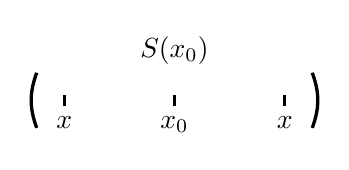
\begin{tikzpicture}[very thick,scale=0.7]
		\tkzInit[xmin=-4, xmax=4, ymin=0, ymax=0]
		\tkzDrawX[thick]
		% \tkzGrid
		\draw (0, -0.1) node[below]{$x_0$}-- (0, 0.1) node[above=7pt]{$\large{S(x_0)}$};
		\draw (-2, -0.1) node[below]{$x$}-- (-2, 0.1);
		\draw (2, -0.1) node[below]{$x$}-- (2, 0.1);
		\draw (-2.5,0.5) to [out=-110, in=110] (-2.5, -0.5);
		\draw (2.5,0.5) to [out=-70, in=70] (2.5, -0.5);
	\end{tikzpicture}\qquad $ \forall x \in S(x_0) \qquad [x_0; x] \text{ или } [x; x_0] $
	\end{center}
	Функции $f(x)$ или $\varphi(x)$ удовлетворяют условию теоремы \textit{Коши} (\textbf{Т.\ref{Коши}}) на $[x_0; x]$.\\
	По теореме \textit{Коши} $\exists\ c \in (x_0; x)\colon$
	\begin{gather*}
		\frac{f(x) - f(x_0)}{\varphi(x)-\varphi(x_0)}=\frac{f'(c)}{\varphi'(c)} \tag{$*$}
	\end{gather*}
	\begin{flalign*}
	& \text{Так как } f(x_0) = 0,\ f(x_0) = 0\ \Rightarrow\ \boxed{\displaystyle\frac{f(x)}{\varphi(x)} = \displaystyle\frac{f'(c)}{\varphi'(c)}} \tag{$*$} &\\
	& \text{Так как } \exists \lim\limits_{x \to x_0} \frac{f'(x)}{\varphi'(x)} = A\colon &
	\end{flalign*}
	\begin{minipage}{16cm}
	\begin{wrapfigure}[2]{r}{0.4\textwidth}
		\vspace{-2.9\topsep}
		\begin{tikzpicture}[very thick,scale=0.7, >=stealth]
			\tkzInit[xmin=-2, xmax=2, ymin=-1, ymax=1]
			% \tkzGrid
			\draw[<->] (-2,0) -- (2,0);
			\draw (-2, -0.2) node[below]{$x_0$}-- (-2, 0.2);
			\draw (2, -0.2) node[below]{$x$}-- (2, 0.2);
			\draw (0, -0.1) node[above]{$c$}-- (0, 0.1);
			\draw[->] (2, -1) to [out=190, in=350] (-2, -1);
			\node at (4, 0) {$\footnotesize{\begin{aligned} &x \to x_0 \\ & c \to x_0 \end{aligned}}$};
		\end{tikzpicture}
	\end{wrapfigure}
	Правая часть $(*)\colon \lim\limits_{c \to x_0} \dfrac{f'(c)}{\varphi'(c)} \xlongequal{\text{4)}} A $
	\end{minipage}\\[1ex] 
	Левая часть $(*)\colon \lim\limits_{x \to x_0} \dfrac{f(x)}{\varphi(x)} = \lim\limits_{c \to x_0}\dfrac{f'(c)}{\varphi'(c)}=A$\\[1ex]
	Получаем, что $\lim\limits_{x\to x_0}\dfrac{f(x)}{\varphi(x)}=\lim\limits_{x \to x_0}\dfrac{f'(x)}{\varphi'(x)} = A$
\end{proof}

\section{Сравните рост показательной, степенной и логарифмической функций на бесконечности.}

Пусть\quad $\begin{aligned}
  & f(x) = x^{n},\ n \in \N         \\
  & g(x) = a^x,\ a>1                \\
  & h(x) = \ln x\qquad 
\end{aligned}\qquad x\to +\infty $
\begin{flalign*}
& \lim_{x\to +\infty} \frac{f(x)}{g(x)} = \lim_{x\to +\infty} \frac{x^n}{a^x} = \left(\frac{\infty}{\infty}\right) \xlongequal{\text{Л-Б}} \lim_{x\to +\infty}\frac{n\cdot x^{n-1}}{a^x\cdot \ln a} = \left(\frac{\infty}{\infty}\right) \xlongequal{\text{Л-Б}} &\\
& \xlongequal{\text{Л-Б}} \underset{n \text{ раз }}{\text{\ldots}} \xlongequal{\text{Л-Б}} \lim_{x\to +\infty}\frac{n\cdot (n-1)\cdot(n-2)\cdot\ldots\cdot 1}{a^x(\ln a)^n}= \frac{n!}{\ln^n a}\cdot \lim_{x\to +\infty}\frac{1}{a^x}=\frac{n!}{\ln^n a}\cdot 0 = 0&
\end{flalign*}
$a^x$ растёт быстрее, чем $x^n$ при $x\to +\infty$ или $x^n = o(a^x)$ при $x\to +\infty$
\begin{flalign*}
& \lim_{x\to +\infty}\frac{h(x)}{f(x)}=\lim_{x\to +\infty}\frac{\ln x}{x^n}=\left(\frac{\infty}{\infty}\right) = \lim_{x\to +\infty}\frac{\frac{1}{x}}{n\cdot x^{n-1}} = \frac{1}{n}\cdot \lim_{x\to +\infty} \frac{1}{x^n}=\frac{1}{n}\cdot 0 = 0 &
\end{flalign*}
$x^n$ растёт быстрее, чем $\ln x$ при $x\to +\infty$ или $\ln x = o(x^n)$ при $x\to +\infty$\\[1ex]
$\left. \begin{array}{lclll}
\text{Вывод:} & 1. & g(x) = a^x & , & a>1\\
& 2. & f(x) = x^n & , & n\in \N\\
& 3. & h(x) = \ln x & & 
\end{array} \right\uparrow\quad x\to +\infty$

\section{Выведите формулу Тейлора с остаточным членом в форме Лагранжа.}

\begin{theorem}
	Пусть функция $y=f(x)$ $(n+1)$ раз дифференцируема в $S(x_0)$,\\
	$\forall x \in S(x_0)\colon f^{(n+1)}(x)\ne0$. Тогда: 
	\begin{gather*}
		\underset{\text{форма Лагранжа}}{\boxed{R_n(x) = \frac{f^{(n+1)}(c)}{(n+1)!}\cdot (x- x_0)^{n+1}}, \text{ где } c \in S(x_0)}
	\end{gather*}
\end{theorem}
\begin{proof}
	$f(x) = P_n(x) + R_n(x)$\\
	Будем искать:
	\begin{gather*}
		R_n(x) = \frac{\varphi(x)}{(n+1)!}\cdot(x-x_0)^{n+1}, \text{ где $\varphi(x)$ -- неизвестная функция}
	\end{gather*}
	Вспомогательная функция:
	\begin{flalign*}
		F(t) &= P_n(t) + R_n(t) - f(x) = &\\
		& = f(t) + \frac{f'(t)}{1!}\cdot(x-t) + \frac{f''(t)}{2!}\cdot(x-t)^2 + \ldots + \frac{f^{(n)}(t)}{n!}\cdot(x-t)^n + &\\
		& + \frac{\varphi(x)}{(n+1)!}\cdot(x-t)^{n+1} - f(x),\quad \text{$t$ -- переменная}&
	\end{flalign*} 
	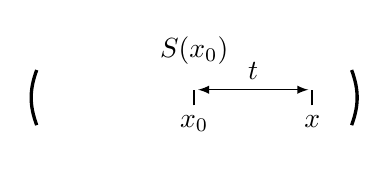
\begin{tikzpicture}[very thick, >=latex]
		\tkzInit[xmin=-2.5, xmax=2.5, ymin=0, ymax=1]
		\tkzDrawX[thick]
		\draw (-2,0.35) to [out=-110, in=110] (-2, -0.35);
		\draw (2,0.35) to [out=-70, in=70] (2, -0.35);
		\draw[thick] (0, -0.1) node[below]{$x_0$}-- (0, 0.1);
		\draw[thick] (1.5, -0.1) node[below]{$x$} -- (1.5, 0.1);
		\draw[thin, <->] (0.05, 0.1) -- (1.45, 0.1) node[midway, above]{$t$};
		\node[above = 8pt] at (0, 0) {$S(x_0)$};
	\end{tikzpicture} \qquad
	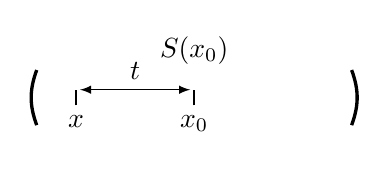
\begin{tikzpicture}[very thick, >=latex]
		\tkzInit[xmin=-2.5, xmax=2.5, ymin=0, ymax=1]
		\tkzDrawX[thick]
		\draw (-2,0.35) to [out=-110, in=110] (-2, -0.35);
		\draw (2,0.35) to [out=-70, in=70] (2, -0.35);
		\draw[thick] (0, -0.1) node[below]{$x_0$}-- (0, 0.1);
		\draw[thick] (-1.5, -0.1) node[below]{$x$} -- (-1.5, 0.1);
		\draw[thin, <->] (-0.05, 0.1) -- (-1.45, 0.1) node[midway, above]{$t$};
		\node[above = 8pt] at (0, 0) {$S(x_0)$};
	\end{tikzpicture}\\
	Функция $F(t)$ удовлетворяет условию теоремы \textit{Ролля} (\textbf{Т.\ref{Ролль}}) на $[x_0; x]\ |\ [x; x_0]$
	\begin{enumerate}
		\item $F(t)$ --- непрерывна на $[x_0; x]\ |\ [x; x_0]$.\\
		По условию функция $f(x)$ $(n+1)$ раз дифференцируема в $S(x_0)\ \Rightarrow$ по теореме \textit{о связи дифференцируемости и непрерывности} (\textbf{Т.\ref{Связь диф. и непр. функции}}):\\
		 $f(t), f'(t), \ldots, f^{(n)}(t)$ --- непрерывны на $[x_0; x]\ |\ [x; x_0]$.\\
		$F(t)$ --- непрерывна на $[x_0; x]\ |\ [x; x_0]$ как сумма непрерывных функций.
		\item $F(t)$ -- дифференцируема на $(x_0; x)\ |\ (x; x_0)$\\
		По условию $y=f(x)$ $(n+1)$ раз дифференцируема в $S(x_0)\ \Rightarrow$\\
		$f(t), f'(t), \ldots, f^{(n)}(t)$ --- дифференцируемы на $(x_0; x)\ |\ (x; x_0)$.\\
		$F(t)$ --- дифференцируема как сумма дифференцируемых функций.
		\item $F(x) = f(x) - f(x) = 0$  
		\begin{flalign*}
			F(x_0) = f(x_0) &+ \frac{f'(x_0)}{1!}\cdot(x-x_0) + \ldots + \frac{f^{(n)}(x_0)}{n!}\cdot(x-x_0)^{n} + &\\
			& + \frac{\varphi(x)}{(n+1)!}\cdot(x - x_0)^{n+1} - f(x) = f(x) - f(x) = 0 &
		\end{flalign*}
		По теореме \textit{Ролля}: $\exists\ c \in (x; x_0)\ |\ c \in (x_0; x)\colon F'(c) = 0$\\
		Вычислим $F'(t)$:
		\begin{flalign*}
			F'(t) = f'(t) &+ \left(\frac{f''(t)}{1!}\cdot(x-t) + \frac{f'(t)}{1!}\cdot(-1)\right) + &\\
			& + \left(\frac{f'''(t)}{2!}\cdot(x-t)^2 + \frac{f''(t)}{2!}\cdot 2 \cdot (x-t) \cdot (-1) \right) + \ldots + &\\
			& + \left(\frac{f^{(n+1)}(t)}{n!}\cdot(x-t)^n + \frac{f^{(n)}(t)}{n!}\cdot n \cdot (x-t)^{n-1}\cdot (-1)\right) + &\\
			& + \frac{\varphi(x)}{(n+1)!}\cdot (n+1) \cdot (x-t)^n \cdot (-1) &
		\end{flalign*}
		\begin{flalign*}
			F'(c) = \frac{f^{(n+1)}(c)}{n!}\cdot (x-c)^n &- \frac{\varphi(x)}{n! \cdot \cancel{(n+1)}}\cdot \cancel{(n+1)} \cdot (x-c)^n = 0 &\\
			\frac{f^{(n+1)}(c)}{n!}\cdot (x-c)^n	&= \frac{\varphi(x)}{n!}\cdot (x-c)^n &\\
			\varphi(x) & = f^{(n+1)}(c),\quad c\in (x_0; x)\ |\ c\in (x; x_0)  &
		\end{flalign*}
		\begin{flalign*}
			& R_n(x) = \frac{f^{(n+1)}(c)}{(n+1)!}\cdot (x-x_0)^{n+1},\quad \forall\ c \in S(x_0) &
		\end{flalign*}
	\end{enumerate}
\end{proof}
Иногда $c = x_0 + \Theta (x-x_0)$\qquad $\Theta$ -- малый параметр \qquad $\Theta \in (0; 1)$

\section{Выведите формулу Тейлора с остаточным членом в форме Пеано.}

\begin{theorem}
	Пусть функция $y=f(x)$ $n$ раз дифференцируема в точке $x_0$, тогда
	\begin{gather*}
		x\to x_0\qquad \boxed{R_n (x) = o\big((x-x_0)^n\big)} \text{ --- форма Пеано.}
	\end{gather*}
\end{theorem}
\begin{proof}
	Формула Тейлора (\textbf{Т.\ref{формула Тейлора}}): \vspace{-\topsep}
	\begin{flalign*}
		 & f(x) = P_n(x) + R_n(x) & \\
		 & R_n(x) = f(x) - P_n(x) &
	\end{flalign*}\vspace{-2\topsep}
  \begin{flalign*}
		&\text{Пусть выполнено условие: } \left\{\begin{aligned}
			        & P_n(x_0) = f(x_0)                     \\
			        & P'_n(x_0) = f'(x_0)                   \\
			        & P''_n(x_0) = f''(x_0)                 \\
			        & \ldots\ldots\ldots\ldots\ldots\ldots  \\
			        & P^{(n)}_n(x_0) = f^{(n)}(x_0)
		       \end{aligned}\right.& \tag{$*$}
	\end{flalign*}
	В силу условия ($*$):
	\begin{align*}
		 & R_n(x_0) = f(x_0) - P_n(x_0) \xlongequal{\text{($*$)}} f(x_0) - f(x_0) = 0 \\
		 & R_n'(x_0) = f'(x_0) - P'_n(x_0) \xlongequal{\text{($*$)}} f'(x_0) - f'(x_0) = 0 \\
		 & \ldots \ldots \ldots \ldots\ldots\ldots\ldots\ldots\ldots\ldots\ldots\ldots\ldots\ldots\ldots\ldots\ldots\ldots \\
		 & R_n^{(n)}(x_0) = f^{(n)}(x_0) - P^{(n)}_n(x_0) \xlongequal{\text{($*$)}} f^{(n)}(x_0) - f^{(n)}(x_0) = 0
	\end{align*}
	Вычислим:
	\begin{flalign*}
		\lim_{x\to x_0}\frac{R_n(x)}{(x-x_0)^n} &= \left(\frac{0}{0}\right) \xlongequal{\text{Л-Б}} \lim_{x\to x_0}\frac{R_n'(x)}{n\cdot(x-x_0)^{n-1}} = \left(\frac{0}{0}\right) \xlongequal{\text{Л-Б}}\ldots =&\\
		& = \lim\limits_{x \to x_0} \frac{R_n^{(n)}(x)}{n\cdot(n-1)\cdot\ldots\cdot 1}= \frac{1}{n!}\lim\limits_{x \to x_0}R_n^{(n)}(x) = \frac{1}{n!}\cdot R_n^{(n)}(x_0) = \frac{1}{n!} \cdot 0 = 0 &
	\end{flalign*}
	Вывод: $R_n(x) = o\big((x-x_0)^n\big)$ при $x \to x_0$
\end{proof}

\section{Выведите формулу Маклорена для функции $y=e^x$ с остаточным членом в форме Лагранжа.}

$y = f(x) = e^x,\quad x_0= 0,\quad f(0) = e^0 = 1$
\begin{flalign*}
	& \left\{ \begin{aligned}
		&f'(x) = e^x\\
		&f''(x) = e^x\\
		&f'''(x) = e^x\\
		&\ldots\ldots\ldots\ldots\\
		&f^{(n)}(x) = e^x
	\end{aligned} \right. \longrightarrow\  \left\{ \begin{aligned}
		&f'(0) = 1\\
		&f''(0) = 1\\
		&f'''(0) = 1\\
		&\ldots\ldots\ldots\ldots\\
		&f^{(n)}(0) = 1
	\end{aligned} \right.&\\
	& e^x = 1 + \frac{1}{1!}\cdot x + \frac{1}{2!}\cdot x^2 + \frac{1}{3!}\cdot x^3 + \ldots + \frac{1}{n!}\cdot x^n + R_n(x)\qquad R_n(x) = o\left(x^n\right) \text{ -- форма Пеано} &\\
	& R_n(x) = \frac{f^{(n+1)} (\Theta x)}{(n+1)!}\cdot x^{n+1} = \frac{e^{\Theta x}}{(n+1)!}\cdot x^{n+1} \text{ -- формула Лагранжа}
\end{flalign*}
	\subsubsection*{Следствия:}
	\begin{enumerate}
		\item $\displaystyle{e^{-x} = 1 - \frac{1}{1!}\cdot x + \frac{1}{2!}\cdot x^2	- \frac{1}{3!}\cdot x^3 + \ldots + \frac{(-1)^n}{n!}\cdot x^n + R_n(x) \qquad n=0, 1, 2, \ldots}$
		\item $\displaystyle{ \sh x = \frac{1}{2}\left(e^x - e^{-x}\right) = \frac{1}{1!}\cdot x + \frac{1}{3!}\cdot x^3 + \frac{1}{5!}\cdot x^5 + \ldots + \frac{1}{(2n+1)!}\cdot x^{2n+1} + R_{2n+2}\quad n=0, 1, 2, \ldots}$
		\item $\displaystyle \ch x = \frac{1}{2}\left(e^x+ e^{-x}\right) = 1 + \frac{1}{2!}\cdot x^2 + \frac{1}{4!}\cdot x^4 + \ldots + \frac{1}{(2n)!}\cdot x^{2n} + R_{2n+1} \qquad n=0,1,2, \ldots$
		\item $\displaystyle a^x = 1+\frac{\ln a}{1!}\cdot x + \frac{\ln^2a}{2!}\cdot x^2 + \ldots + \frac{\ln^n a}{n!}\cdot x^n + R_n(x)\qquad n=0, 1, 2,\ldots$
		\item $\displaystyle \sh^2 x = \left(\frac{e^x - e^{-x}}{2}\right)^2 = \frac{1}{4}\cdot \left(e^{2x} - 2 + e^{-2x}\right)  = \frac{1}{2}\cdot \frac{e^{2x} + e^{-2x}}{2} - \frac{1}{2} = \frac{1}{2}\cdot (\ch 2x - 1) $
		\item $\displaystyle \ch^2 x = \left(\frac{e^x + e^{-x}}{2}\right)^2 = \frac{1}{4}\cdot \left(e^{2x}+ 2 + e^{-2x}\right) = \frac{1}{2} \cdot \frac{e^{2x} + e^{-2x}}{2} + \frac{1}{2} = \frac{1}{2}\cdot \left(\ch 2x + 1\right) $
	\end{enumerate}

\section{Выведите формулу Маклорена для функции $y = \sin x$ с остаточным членом в форме Лагранжа.}

$y = f(x) = \sin x,\ x_0=0$
\begin{flalign*}
	& f(0) = \sin 0 = 0 &\\
	&\left\{ \begin{aligned}
		f'(x) &= \cos x = \sin \left(x + 1\cdot \frac{\pi}{2}\right)\\[1ex]
		f''(x) &= -\sin x = \sin \left(x + 2\cdot \frac{\pi}{2}\right)\\[1ex]
		f'''(x) &= -\cos x = \sin \left(x + 3\cdot \frac{\pi}{2}\right)\\[1ex]
		f^{(IV)}(x) &= \sin x = \sin \left(x + 4\cdot \frac{\pi}{2}\right)\\[1ex]
		f^{(V)}(x) &= \cos x = \sin \left(x + 5\cdot \frac{\pi}{2}\right)\\
		\ldots\ldots&\ldots\ldots\ldots\ldots\ldots\ldots\ldots\ldots\\
		f^{(n)}(x) &= \sin \left(x + n\cdot \frac{\pi}{2}\right) \\
	\end{aligned}\right. \ \longrightarrow\ \left\{\begin{aligned}
		f'(0) &= 1 \\[2.9ex]
		f''(0) &= 0 \\[2.9ex]
		f'''(0) &= -1 \\[2.9ex]
		f^{(IV)}(0) &= 0 \\[2.9ex]
		f^{(V)}(0) &= 1 \\
		\ldots\ldots&\ldots\ldots\ldots \\
		f^{(n)}(0) &= \sin \frac{\pi n}{2} \\
	\end{aligned} \right. &\\[1ex]
	& \sin x = 0 + \frac{1}{1!}\cdot x + \frac{0}{2!}\cdot x^2 - \frac{1}{3!}\cdot x^3 + \frac{0}{4!}\cdot x^4 + \frac{1}{5!}\cdot x^5 + \ldots + \frac{\sin \dfrac{\pi n}{2}}{n!}\cdot x^n + R_n(x)\quad n = 2k,\ k\in \N&\\[1ex]
	& \sin \frac{\pi n}{2} = \left\{ \begin{aligned}
		0,\quad &n = 2k,\ k \in \N \\
		(-1)^{k+1},\quad &n = 2k -1,\ k \in \N
	\end{aligned} \right. &\\[1ex]
	& \sin x = \frac{1}{1!}\cdot x - \frac{1}{3!}\cdot x^3 + \frac{1}{5!}\cdot x^5 + \ldots + \frac{(-1)^{k+1}}{(2k-1)!}\cdot x^{2k-1} + R_{2k}(x) &\\
	& R_{2k}(x) = o\left(x^{2k}\right) &
\end{flalign*}\vspace{-4\topsep}
\begin{flalign*}
	R_{2k}(x) &= R_n(x) = \frac{f^{(n+1)}(\Theta x)}{(n+1)!}\cdot x^{n+1} = \frac{f^{(2k+1)}(\Theta x)}{(2k+1)!} \cdot x^{2k+1} = \frac{\sin \left(\Theta x + (2k+1)\cdot \dfrac{\pi}{2}\right)}{(2k+1)!}\cdot x^{2k+1}= &\\
	& = \frac{\sin \left(\Theta x + \pi k + \dfrac{\pi}{2}\right)}{(2k+1)!}\cdot x^{2k+1} = \frac{\cos \left(\Theta x + \pi k \right)}{(2k+1)!}\cdot x^{2k+1} = \frac{(-1)^k \cdot \cos \Theta x }{(2k+1)!}\cdot x^{2k+1} &\\
\end{flalign*} 
\begin{tikzpicture}[scale=1, very thick]
	\tkzInit[xmin=-2, xmax=2, ymin=-2, ymax=1.5]
	\tkzDrawX[thick] \tkzDrawY[thick]
	\tkzDefPoint(0.8, {sqrt(1.5**2 - 0.8**2)}){plus}
	\tkzDefPoint(-0.8, {-sqrt(1.5**2 - 0.8**2)}){minus}
	\draw (0, 0) circle (1.5);
	\tkzDrawPoint[size = 3pt](plus)
	\tkzDrawPoint[size = 3pt](minus)
	\draw (minus) -- (-0.8, 0) node[midway, right]{\textcircled{$-$}};
	\draw (plus) -- (0.8, 0) node[midway, left]{\textcircled{$+$}};
	\node[above left] at (-1.5, 0) {$\pi$};
	\node[above right] at (1.5, 0) {$2\pi$};
	\node[above] at (-0.8, 0) {$\cos x$};
	\node at (3, 1.5) {$k=1,2,\ldots$};
\end{tikzpicture}

\section{Выведите формулу Маклорена для функции $y = \cos x$ с остаточным членом в форме Лагранжа.}

$y = f(x) = \cos x,\ x_0=0,\ f(0) = \cos 0 = 1$
\begin{flalign*}
	& f(0) = \cos 0 = 1 &\\
	&\left\{ \begin{aligned}
		f'(x) &= -\sin x= \cos \left(x + 1\cdot \frac{\pi}{2}\right)\\[1ex]
		f''(x) &= -\cos x = \cos \left(x + 2\cdot \frac{\pi}{2}\right)\\[1ex]
		f'''(x) &= \sin x = \cos \left(x + 3\cdot \frac{\pi}{2}\right)\\[1ex]
		f^{(IV)}(x) &= \cos x = \cos \left(x + 4\cdot \frac{\pi}{2}\right)\\[1ex]
		f^{(V)}(x) &= -\sin x = \cos \left(x + 5\cdot \frac{\pi}{2}\right)\\
		\ldots\ldots&\ldots\ldots\ldots\ldots\ldots\ldots\ldots\ldots\\
		f^{(n)}(x) &= \cos \left(x + n\cdot \frac{\pi}{2}\right) \\
	\end{aligned}\right. \ \longrightarrow\ \left\{\begin{aligned}
		f'(0) &= 0 \\[2.9ex]
		f''(0) &= -1 \\[2.9ex]
		f'''(0) &= 0 \\[2.9ex]
		f^{(IV)}(0) &= 1 \\[2.9ex]
		f^{(V)}(0) &= 0 \\
		\ldots\ldots&\ldots\ldots\ldots \\
		f^{(n)}(0) &= \cos \frac{\pi n}{2} \\
	\end{aligned} \right. &\\[1ex]
	& \cos x = 1 + \frac{0}{1!}\cdot x - \frac{1}{2!}\cdot x^2	+ \frac{0}{3!}\cdot x^3 + \frac{1}{4!}\cdot x^4 + \frac{0}{5!}\cdot x^5 + \ldots + \frac{\cos \dfrac{\pi n}{2}}{n!}\cdot x^n + R_n(x)&\\[1ex]
	& \cos \frac{\pi n}{2} = \left\{ \begin{aligned}
		0,\quad &n = 2k-1,\ k \in \N\\
		(-1)^{k},\quad &n = 2k,\ k \in \N
	\end{aligned} \right. &\\[1ex]
	& \cos x = 1 - \frac{1}{2!}\cdot x^2 + \frac{1}{4!}\cdot x^4 + \ldots + \frac{(-1)^k}{(2k)!}\cdot x^{2k} + R_{2k+1}(x)&\\
	& R_{2k+1} (x) = o\left(x^{2k+1}\right)&
\end{flalign*}\vspace{-4\topsep}
\begin{flalign*}
	R_{2k+1}(x) &= R_n(x) = \frac{f^{(n+1)}(\Theta x)}{(n+1)!}\cdot x^{n+1} = \frac{f^{(2k+2)}(\Theta x)}{(2k+2)!}\cdot x^{2k+2} = \frac{\cos \left(\Theta x + (2k+2)\cdot \dfrac{\pi}{2}\right)}{(2k+2)!}\cdot x^{2k+2} = &\\
	& = \frac{\cos (\Theta x + \pi k + \pi)}{(2k+2)!} \cdot x^{2k+2} = \frac{- \cos (\Theta x + \pi k)}{(2k+2)!} \cdot x^{2k+2} = \frac{(-1) \cdot (-1) \cdot \cos \Theta x}{(2k+2)!} \cdot x^{2k+2} = &\\
	& = \frac{(-1)^{k+1}\cdot \cos \Theta x}{(2k+2)!} \cdot x^{2k+2} &
\end{flalign*}
\begin{tikzpicture}[scale=1, very thick]
	\tkzInit[xmin=-2, xmax=2, ymin=-2, ymax=1.5]
	\tkzDrawX[thick] \tkzDrawY[thick]
	\tkzDefPoint(0.8, {sqrt(1.5**2 - 0.8**2)}){plus}
	\tkzDefPoint(-0.8, {-sqrt(1.5**2 - 0.8**2)}){minus}
	\draw (0, 0) circle (1.5);
	\tkzDrawPoint[size = 3pt](plus)
	\tkzDrawPoint[size = 3pt](minus)
	\draw (minus) -- (-0.8, 0) node[midway, right]{\textcircled{$-$}};
	\draw (plus) -- (0.8, 0) node[midway, left]{\textcircled{$+$}};
	\node[above left] at (-1.5, 0) {$\pi$};
	\node[above right] at (1.5, 0) {$2\pi$};
	\node[above] at (-0.8, 0) {$\cos x$};
	\node[below] at (0.8, 0) {$\cos x$};
	\node at (3, 1.5) {$k=1,2,\ldots$};
\end{tikzpicture}

\section{Выведите формулу Маклорена для функции \mbox{$y = \ln(1 + x)$} с остаточным членом в форме Лагранжа.}

$ y= f(x) = \ln (1+x) \qquad x_0 = 0 \qquad f(0) = \ln 1 = 0$
\begin{flalign*}
	&\left\{ \begin{aligned}
		f'(x) &= \frac{1}{1+x} = (1+x)^{-1} \\
		f''(x) &= (-1)\cdot (1+x)^{-2} \\
		f'''(x) &= (-1) \cdot (-2) \cdot (1+x)^{-3} \\
		f^{(IV)}(x) &= (-1) \cdot (-2) \cdot (-3) \cdot (1+x)^{-4} \\
		\ldots\ldots&\ldots\ldots\ldots\ldots\ldots\ldots\ldots\ldots\ldots\ldots\\
		f^{(n)}(x) &= (-1)^{n+1} \cdot (n-1)! \cdot (1+x)^{-n} \\
	\end{aligned}\right. \ \longrightarrow\ \left\{\begin{aligned}
		f'(0) &= 1 = 0! \\[1.2ex]
		f''(0) &= -1 \cdot (-1)\cdot 1! \\
		f'''(0) &= 2 = 2! \\
		f^{(IV)}(0) &= (-1) \cdot 3! \\
		\ldots\ldots&\ldots\ldots\ldots \\
		f^{(n)}(0) &= (-1)^{n+1} \cdot (n-1)! \\
	\end{aligned} \right. &\\[1ex]
	& \ln (1+x) = 0 + \frac{0!}{1!}\cdot x - \frac{1!}{2!}\cdot x^2 + \frac{2!}{3!}\cdot x^3 - \frac{3!}{4!}\cdot x^4 + \ldots + \frac{(-1)^{n+1}\cdot (n-1)!}{n!}\cdot x^n + R_n(x) &\\
	& n! = (n-1)! \cdot n &\\[-0.5ex]
	& \ln (1+x) = \frac{1}{1}\cdot x - \frac{1}{2}\cdot x^2 + \frac{1}{3}\cdot x^3 - \ldots + \frac{(-1)^{n+1}}{n}\cdot x^n + R_n(x) &\\
	& R_n(x) = o\left(x^n\right) \text{ --  форма Пеано}&\\
	& \begin{aligned} R_n(x) = \frac{f^{(n+1)} (\Theta x)}{(n+1)!}\cdot x^{n+1} = \frac{(-1)^{n+2}\cdot n! \cdot (1+\Theta x)^{-(n+1)}}{(n+1)!}\cdot x^{n+1} = & \frac{(-1)^{n+2}\cdot (1+ \Theta x)^{-(n+1)}}{n+1}\cdot x^{n+1} \\ & \text{ форма Лагранжа} \end{aligned} &
\end{flalign*}

\section{Выведите формулу Маклорена для функции \mbox{$y = (1 + x)^\alpha$} с остаточным членом в форме Лагранжа.}

$f(x) = (1+x)^\alpha,\quad \alpha \in \R$\\
$x_0 = 0$ \hspace{10.4cm} $f(0)=1$ \vspace*{-\topsep}
\begin{flalign*}
	& \left\{ \begin{aligned}
		f'(x) &= \alpha \cdot (1 + x)^{\alpha - 1} \\
		f''(x) &= \alpha\cdot (\alpha - 1) \cdot (1 + x)^{\alpha - 2}\\
		f'''(x) &=  \alpha\cdot (\alpha - 1) \cdot (\alpha - 2) \cdot (1 + x)^{\alpha - 3} \\
		\ldots\ldots&\ldots\ldots\ldots\ldots\ldots\ldots\ldots\ldots\ldots\ldots\ldots\ldots\ldots\ldots\\
		f^{(n)}(x) &= \alpha\cdot (\alpha - 1) \cdot  \ldots \cdot (\alpha - (n-1))\cdot (1+x)^{\alpha - n}
	\end{aligned}\right.\ \longrightarrow\ \left\{\begin{aligned}
		f'(0) &= \alpha \\
		f''(0) &= \alpha \cdot (\alpha - 1) \\
		f'''(0) &= \alpha \cdot (\alpha - 1) \cdot (\alpha - 2) \\
		\ldots\ldots&\ldots\ldots\ldots\ldots\ldots\ldots\ldots\ldots\ldots\ldots \\
		f^{(n)}(0) &= \alpha \cdot (\alpha - 1) \cdot \ldots \cdot (\alpha - (n-1)) \\
	\end{aligned} \right. &\\
	& \hspace{2pt} f^{(n+1)}(x) = \alpha \cdot (\alpha - 1) \cdot \ldots \cdot (\alpha - n)\cdot (1+x)^{\alpha - (n+1)} &\\
	& f(x) = f(0) + \frac{f'(0)}{1!}\cdot x + \frac{f''(0)}{2!}\cdot x^2 + \ldots + \frac{f^{(n)}(0)}{n!}\cdot x^n + R_n(x) &\\[1ex]
	& \begin{aligned} (1+x)^\alpha = 1 + \frac{\alpha}{1!} \cdot x + \frac{\alpha \cdot (\alpha - 1)}{2!}\cdot x^2 & + \frac{\alpha \cdot (\alpha - 1) \cdot (\alpha - 2)}{3!}\cdot x^3 + \ldots + \\
		& + \frac{\alpha \cdot (\alpha - 1) \cdot \ldots \cdot \big(\alpha - (n-1)\big)}{n!}\cdot x^n  + R_n(x) \end{aligned} &\\
	& R_n(x) = o\left(x^n\right) \text{ --- форма Пеано} &\\
	& R_n(x) = \frac{f^{(n+1)} (\Theta x)}{(n+1)!}\cdot x^{n+1} = \frac{\alpha \cdot (\alpha - 1) \cdot \ldots \cdot (\alpha - n)}{(n+1)!}\cdot (1 + \Theta x)^{\alpha - (n+1)} \cdot x^{n+1} \text{ --- форма Лагранжа} & 
\end{flalign*}

\section{Сформулируйте и докажите необходимое и достаточное условие неубывания дифференцируемой функции.}

\begin{theorem}[Необходимое и достаточное условие невозрастания | неубывания дифференцируеммой функции]
	Дифференцируемая на интервале $(a;b)$ функция $y=f(x)$ не возрастает (не убывает) на этом интервале тогда и только тогда, когда $\forall\ x \in (a;b)\colon$
	\[ f'(x) \le 0\quad \Big(f'(x) \ge 0\Big) \]
\end{theorem}
\begin{proof}[][Необходимость]
	\textbf{Дано}: $y=f(x)$ не \stackon{возрастает}{\footnotesize{(убывает)}} на $(a;b)$\\
	\textbf{Доказать}: $\forall x \in (a;b)\colon f'(x) \overset{\scriptsize{\big(\ge \big)}}{\le} 0$\\
	$\forall x \in (a;b)$\\
	$\Delta x$ --- приращение аргумента\\
	$x \to x + \Delta x$\\
	$\Delta y = y(x + \Delta x) - y(x)$ --- приращение функции\\
	Случаи:
	\begin{enumerate}
		\item $\Delta x > 0$\\
		      Так как $y=f(x)$ не \stackon{возрастает}{\footnotesize{(убывает)}} на $(a;b)$: \vspace{-\topsep}
		      \begin{align*}
			                 & y(x+\Delta x) \overset{\scriptsize{\big(\ge \big)}}{\le} y(x)       \\
			      \Delta y = & y(x + \Delta x) - y(x) \overset{\scriptsize{\big(\ge \big)}}{\le} 0
		      \end{align*} \vspace{-\topsep}
		      Тогда:
		      \begin{gather*}
			      \boxed{\frac{\Delta y}{\Delta x} = \left(\frac{-}{+}\right) \overset{\scriptsize{\big(\ge \big)}}{\le} 0}
		      \end{gather*}
		\item $\Delta x < 0$\\
		      Так как $y=f(x)$ не \stackon{возрастает}{\footnotesize{(убывает)}} на $(a;b)$: \vspace{-\topsep}
		      \begin{align*}
			                 & y(x+\Delta x) \overset{\scriptsize{\big(\le \big)}}{\ge} y(x)       \\
			      \Delta y = & y(x + \Delta x) - y(x) \overset{\scriptsize{\big(\le \big)}}{\ge} 0
		      \end{align*} \vspace{-\topsep}
		      Тогда:
		      \begin{gather*}
			      \boxed{\frac{\Delta y}{\Delta x} = \left(\frac{+}{-}\right) \overset{\scriptsize{\big(\ge \big)}}{\le} 0}
		      \end{gather*}
	\end{enumerate}
	По теореме \textit{о предельном переходе в неравенстве} (\textbf{Т.\ref{Предельный переход в неравенстве}}):
	\begin{gather*}
		\lim\limits_{\Delta x \to 0} \frac{\Delta y}{\Delta x} \overset{\scriptsize{\big(\ge \big)}}{\le} 0
	\end{gather*}
	По определению производной (\textbf{опр.\ref{опр: производная функции}}): $f'(x) \overset{\scriptsize{\big(\ge \big)}}{\le} 0$
\end{proof}
\begin{proof}[][Достаточность]
	\textbf{Дано}: $\forall x \in (a;b)\colon f'(x) \overset{\scriptsize{\big(\ge \big)}}{\le} 0$\\
	\textbf{Доказать}: $y=f(x)$ не \stackon{возрастает}{\footnotesize{(убывает)}} на $(a;b)$\\
	$\forall\ x_1, x_2 \in (a;b)\colon x_2 > x_1$\\
	Рассмотрим $[x_1; x_2]$.\\
	Функция $y=f(x)$ на $[x_1, x_2]$ удовлетворяет условиям теоремы \textit{Лагранжа} (\textbf{Т.\ref{Лагранж}}):
	\begin{enumerate}
		\item Непрерывность на $[x_1; x_2]$\\
		      По условию $y=f(x)$ дифференцируема на $(a;b)$. По теореме \textit{о связи дифференцируемости и непрерывности функции} (\textbf{Т.\ref{Связь диф. и непр. функции}}) $\Rightarrow\ y=f(x)$ непрерывна на $[x_1; x_2]$.
		\item Дифференцируемость на $(x_1; x_2)$\\
		      Так как по условию. $y=f(x)$ дифференцируема на $(a;b)$, по теореме \textit{Лагранжа} $\exists\ c \in (x_1; x_2)$: \vspace{-\topsep}
		      \begin{gather*}
			      f'(c) = \frac{f(x_2) - f(x_1)}{x_2 - x_1}
		      \end{gather*}
		      Так как $x_2 > x_1$, то $x_2 - x_1 > 0$.\\
		      По условию $f'(x) \overset{\scriptsize{\big(\ge \big)}}{\le} 0$, $\forall x \in (a;b)\ \Rightarrow\ f'(c) \overset{\scriptsize{\big(\ge \big)}}{\le} 0$.\\
		      Тогда:
		      \begin{gather*}
			      f'(c) = \frac{f(x_2) - f(x_1)}{x_2 - x_1} \overset{\scriptsize{\big(\ge \big)}}{\le} 0\ \Rightarrow\ f(x_2) - f(x_1) \overset{\scriptsize{\big(\ge \big)}}{\le} 0 \text{ при } x_2 > x_1
		      \end{gather*}
	\end{enumerate} \vspace{-\topsep}
	$f(x_2) \overset{\scriptsize{\big(\ge \big)}}{\le} f(x_1)$ при $x_2 > x_1\ \Rightarrow$ по \stackon{определению}{\footnotesize{(\textbf{опр.\ref{опр: невозрастающая функция} (\ref{опр: неубывающая функция})})}} функция $y=f(x)$ не \stackon{возрастает}{\footnotesize{(убывает)}} на $(a;b)$.
\end{proof} \vspace{-11pt}
\begin{note}[\textbf{к доказательству}]
	Записи в скобках над словом или символом --- это то, что используется в доказательстве для неубывания.
\end{note}

\newpage
\section{Сформулируйте и докажите необходимое и достаточное условие невозрастания дифференцируемой функции.}

\begin{theorem}[Необходимое и достаточное условие невозрастания | неубывания дифференцируеммой функции]
	Дифференцируемая на интервале $(a;b)$ функция $y=f(x)$ не возрастает (не убывает) на этом интервале тогда и только тогда, когда $\forall\ x \in (a;b)\colon$
	\[ f'(x) \le 0\quad \Big(f'(x) \ge 0\Big) \]
\end{theorem}
\begin{proof}[][Необходимость]
	\textbf{Дано}: $y=f(x)$ не \stackon{возрастает}{\footnotesize{(убывает)}} на $(a;b)$\\
	\textbf{Доказать}: $\forall x \in (a;b)\colon f'(x) \overset{\scriptsize{\big(\ge \big)}}{\le} 0$\\
	$\forall x \in (a;b)$\\
	$\Delta x$ --- приращение аргумента\\
	$x \to x + \Delta x$\\
	$\Delta y = y(x + \Delta x) - y(x)$ --- приращение функции\\
	Случаи:
	\begin{enumerate}
		\item $\Delta x > 0$\\
          Так как $y=f(x)$ не \stackon{возрастает}{\footnotesize{(убывает)}} на $(a;b)$: \vspace{-\topsep}
          \begin{align*}
            & y(x+\Delta x) \overset{\scriptsize{\big(\ge \big)}}{\le} y(x) \\
            \Delta y = & y(x + \Delta x) - y(x) \overset{\scriptsize{\big(\ge \big)}}{\le} 0
          \end{align*} \vspace{-\topsep}
          Тогда:
          \begin{gather*}
            \boxed{\frac{\Delta y}{\Delta x} = \left(\frac{-}{+}\right) \overset{\scriptsize{\big(\ge \big)}}{\le} 0}
          \end{gather*}
    \item $\Delta x < 0$\\
          Так как $y=f(x)$ не \stackon{возрастает}{\footnotesize{(убывает)}} на $(a;b)$: \vspace{-\topsep}
          \begin{align*}
            & y(x+\Delta x) \overset{\scriptsize{\big(\le \big)}}{\ge} y(x) \\
            \Delta y = & y(x + \Delta x) - y(x) \overset{\scriptsize{\big(\le \big)}}{\ge} 0
          \end{align*} \vspace{-\topsep}
          Тогда:
          \begin{gather*}
            \boxed{\frac{\Delta y}{\Delta x} = \left(\frac{+}{-}\right) \overset{\scriptsize{\big(\ge \big)}}{\le} 0}
          \end{gather*}
	\end{enumerate}
	По теореме \textit{о предельном переходе в неравенстве} (\textbf{Т.\ref{Предельный переход в неравенстве}}):
	\begin{gather*}
		\lim\limits_{\Delta x \to 0} \frac{\Delta y}{\Delta x} \overset{\scriptsize{\big(\ge \big)}}{\le} 0
	\end{gather*}
	По определению производной (\textbf{опр.\ref{опр: производная функции}}): $f'(x) \overset{\scriptsize{\big(\ge \big)}}{\le} 0$
\end{proof}
\begin{proof}[][Достаточность]
	\textbf{Дано}: $\forall x \in (a;b)\colon f'(x) \overset{\scriptsize{\big(\ge \big)}}{\le} 0$\\
	\textbf{Доказать}: $y=f(x)$ не \stackon{возрастает}{\footnotesize{(убывает)}} на $(a;b)$\\
	$\forall\ x_1, x_2 \in (a;b)\colon x_2 > x_1$\\
	Рассмотрим $[x_1; x_2]$.\\
	Функция $y=f(x)$ на $[x_1, x_2]$ удовлетворяет условиям теоремы \textit{Лагранжа} (\textbf{Т.\ref{Лагранж}}):
	\begin{enumerate}
		\item Непрерывность на $[x_1; x_2]$\\
		      По условию $y=f(x)$ дифференцируема на $(a;b)$. По теореме \textit{о связи дифференцируемости и непрерывности функции} (\textbf{Т.\ref{Связь диф. и непр. функции}}) $\Rightarrow\ y=f(x)$ непрерывна на $[x_1; x_2]$.
		\item Дифференцируемость на $(x_1; x_2)$\\
		      Так как по условию. $y=f(x)$ дифференцируема на $(a;b)$, по теореме \textit{Лагранжа} $\exists\ c \in (x_1; x_2)$: \vspace{-\topsep}
		      \begin{gather*}
			      f'(c) = \frac{f(x_2) - f(x_1)}{x_2 - x_1}
		      \end{gather*}
		      Так как $x_2 > x_1$, то $x_2 - x_1 > 0$.\\
		      По условию $f'(x) \overset{\scriptsize{\big(\ge \big)}}{\le} 0$, $\forall x \in (a;b)\ \Rightarrow\ f'(c) \overset{\scriptsize{\big(\ge \big)}}{\le} 0$.\\
		      Тогда:
		      \begin{gather*}
			      f'(c) = \frac{f(x_2) - f(x_1)}{x_2 - x_1} \overset{\scriptsize{\big(\ge \big)}}{\le} 0\ \Rightarrow\ f(x_2) - f(x_1) \overset{\scriptsize{\big(\ge \big)}}{\le} 0 \text{ при } x_2 > x_1
		      \end{gather*}
	\end{enumerate} \vspace{-\topsep}
	$f(x_2) \overset{\scriptsize{\big(\ge \big)}}{\le} f(x_1)$ при $x_2 > x_1\ \Rightarrow$ по \stackon{определению}{\footnotesize{(\textbf{опр.\ref{опр: невозрастающая функция} (\ref{опр: неубывающая функция})})}} функция $y=f(x)$ не \stackon{возрастает}{\footnotesize{(убывает)}} на $(a;b)$.
\end{proof} \vspace{-11pt}
\begin{note}[\textbf{к доказательству}]
	Записи в скобках над словом или символом --- это то, что используется в доказательстве для неубывания.
\end{note}

\newpage
\section{Сформулируйте и докажите первое достаточное условие экстремума (по первой производной).}

\begin{theorem}[Первый достаточный признак локального экстремума]
	Пусть $y=f(x)$ непрерывна в $S(x_0)$, где $x_0$ --- критическая точка 1-го порядка; дифференцируема в $\mathring{S}(x_0)$. Тогда если производная функции меняет свой знак при переходе через точку $x_0$, то $x_0$ --- точка экстремума. Причём:
	\begin{enumerate}
		\item если при $x < x_0\colon f'(x) > 0$, а при $x > x_0\colon f'(x) < 0$, то $x_0$ --- точка максимума;
		\item если при $x < x_0\colon f'(x) < 0$, а при $x > x_0\colon f'(x) > 0$, то $x_0$ --- точка минимума.
	\end{enumerate}
\end{theorem}
\begin{proof}
	$\forall x \in S(x_0)$.\\
	$\bullet$ Пусть $x > x_0$. Рассмотрим $[x_0; x]$. \\
	Тогда функция $y=f(x)$ удовлетворяет условиям теоремы \textit{Лагранжа} (\textbf{Т.\ref{Лагранж}}):
	\begin{enumerate}
		\item непрерывна на $[x_0; x]$\\
		      По условию функция непрерывна в $S(x_0)\ \Rightarrow\ y=f(x)$ непрерывна на $[x_0; x]$.
		\item дифференцируема на $(x_0; x)$\\
		      По условию $y=f(x)$ дифференцируема в $\mathring{S}(x_0)\ \Rightarrow\ y=f(x)$ дифференцируема на $(x_0; x)$.
	\end{enumerate}
	По теореме \textit{Лагранжа} $\displaystyle \exists\ c \in (x_0; x)\colon f(c) = \frac{f(x) - f(x_0)}{x - x_0}$\\
	Так как $x > x_0$, то $x - x_0 > 0$.\\
	По условию 1) при $x > x_0\colon f'(x) \overset{\scriptsize{\big(>\big)}}{<} 0\ \Rightarrow$
	\begin{gather*}
		\Rightarrow\ f'(c) = \frac{f(x) - f(x_0)}{x - x_0} \overset{\scriptsize{\big(>\big)}}{<} 0\ \Rightarrow\ f(x) - f(x_0) \overset{\scriptsize{\big(>\big)}}{<} 0\ \Rightarrow\ f(x) \overset{\scriptsize{\big(>\big)}}{<} f(x_0)
	\end{gather*}
	По \stackon{определению}{\footnotesize{(\textbf{опр.\ref{опр: строгий максимум} (\ref{опр: строгий минимум})})}} строгого \stackon{максимума}{\footnotesize{(минимума)}}, $x_0$ --- точка \stackon{максимума}{\footnotesize{(минимума)}}.\\
	$\bullet$ Пусть $x<x_0$, тогда рассматриваем $[x; x_0]$.\\
	$y=f(x)$ на $[x; x_0]$ удовлетворяет теореме \textit{Лагранжа}.\\[1ex]
	По теореме \textit{Лагранжа}: $\displaystyle \exists\ c \in (x; x_0)\colon f'(c) = \frac{f(x_0) - f(x)}{x_0 - x}$\\[1ex]
	Так как $x < x_0$, то $x - x_0 < 0\ \Rightarrow\ x_0-x > 0$.\\
	По условию 1) при $x < x_0\colon f'(x) \overset{\scriptsize{\big(<\big)}}{>} 0\ \Rightarrow$
	\begin{gather*}
		\Rightarrow\ f'(c) = \frac{f(x_0) - f(x)}{x_0 - x} \overset{\scriptsize{\big(<\big)}}{>} 0\ \Rightarrow\ f(x_0) - f(x) \overset{\scriptsize{\big(<\big)}}{>} 0\ \Rightarrow\ f(x_0) \overset{\scriptsize{\big(<\big)}}{>} f(x)
	\end{gather*}
	По определению строго локального \stackon{максимума}{\footnotesize{(минимума)}}, $x_0$ --- точка строгого локального\\[1ex]
	\stackon{максимума}{\footnotesize{(минимума)}} $\Rightarrow\ \forall x \in S(x_0)\colon x_0$ --- точка строгого локального \stackon{максимума}{\footnotesize{(минимума)}}.
\end{proof} \vspace{-11pt}
\begin{note}[{\textbf{к доказательству}}]
	Записи в скобках над словом или символом --- это то, что используется в доказательстве для случая строго локального минимума.
\end{note}

\section{Сформулируйте и докажите второе достаточное условие экстремума (по второй производной).}

\begin{theorem}[Второй достаточный признак локального экстремума]
	Пусть функция $y=f(x)$ дважды дифференцируема в точке $x_0$ и $f'(x_0) = 0$. Тогда:
	\begin{enumerate}
		\item если $f''(x_0) < 0$, то $x_0$ --- точка строгого максимума;
		\item если $f''(x_0) > 0$, то $x_0$ --- точка строгого минимума.
	\end{enumerate}
\end{theorem}
\begin{proof}
	Представим функцию $y=f(x)$ в $S(x_0)$ по формуле Тейлора:
	\begin{align*}
		f(x) = f(x_0) + \frac{f'(x_0)}{1!}\cdot (x-x_0) +  \frac{f''(x_0)}{2!}\cdot (x-x_0)^2 + o\left((x-x_0)^2\right)
	\end{align*}
	Так как $f'(x_0) = 0$, то:
	\begin{align*}
		f(x)          & = f(x_0) + \frac{f''(x_0)}{2!}\cdot (x-x_0)^2 + o\left((x-x_0)^2\right) \\
		f(x) - f(x_0) & = \frac{f''(x_0)}{2!}\cdot (x-x_0)^2 + o\left((x-x_0)^2\right)
	\end{align*}
	Знак $f(x) - f(x_0)$ определяет $f''(x_0)$, так как $o\left((x-x_0)^2\right)$ --- б.м.ф. при $x\to x_0$.\\
	Тогда: \vspace{-8pt}
	\begin{enumerate}
		\item если $f''(x_0) < 0$, то $f(x) - f(x_0) < 0\ \Rightarrow\ f(x) < f(x_0),\ \forall x \in S(x_0)$, по \stackon{определению}{\footnotesize{(\textbf{опр.\ref{опр: строгий максимум}})}} строгого локального максимума $x_0$ --- точка строго локального максимума;
		\item если $f''(x_0) > 0$, то $f(x) - f(x_0) > 0\ \Rightarrow\ f(x) > f(x_0)\quad \forall x \in S(x_0)$, по \stackon{определению}{\footnotesize{(\textbf{опр.\ref{опр: строгий минимум}})}} строгого локального минимума $x_0$ --- точка строгого локального минимума.
	\end{enumerate}
\end{proof}

\newpage
\section{Сформулируйте и докажите достаточное условие выпуклости функции.}

\begin{theorem}[Достаточное условие выпуклости графика функции]\hlabel{Достаточное условие выпуклости}
	Пусть функция $y=f(x)$ дважды дифференцируема на интервале $(a;b)$. Тогда:
	\begin{enumerate}\vspace{-0.5ex}
		\item Если $f''(x) < 0,\ \forall x \in (a;b)$, то график функции выпуклый вверх на этом интервале.\vspace{-1.5ex}
		\item Если $f''(x) > 0,\ \forall x \in (a;b)$, то график функции выпуклый вниз на этом интервале.
	\end{enumerate}
\end{theorem}
\begin{proof}
	$\forall x_0 \in (a;b),\ y_0=f(x_0)\ \Rightarrow\ M_0\big(x_0, f(x_0)\big)$\\
	В точке $M_0$ построим касательную к графику функции $y=f(x)$:
	\begin{align*}
		\underset{\text{уравнение касательной}}{y-y_0 = y'(x_0)(x-x_0)}\ \Rightarrow\ \boxed{y_{\text{к}} = f(x_0) + f'(x_0)(x-x_0)}
	\end{align*}
	Представим функцию $y=f(x)$ по формуле Тейлора с остаточным членом в форме Лагранжа:
	\begin{gather*}
		\boxed{f(x) = f(x_0) + \frac{f'(x_0)}{1!}\cdot (x-x_0) + \frac{f''(c)}{2!}\cdot (x-x_0)^2}\quad \forall c \in \mathring{S}(x_0)
	\end{gather*}
	Из представления для функции вычитаем уравнение касательной:
	\begin{align*}
		f(x) - y_{\text{к}} &= \cancel{f(x_0)} + \bcancel{\frac{f'(x_0)}{1!}\cdot (x-x_0)} + \frac{f''(c)}{2!}\cdot (x-x_0)^2 - \cancel{f(x_0)} - \bcancel{f'(x_0)(x-x_0)}\\
		f(x) - y_{\text{к}} &= \frac{f''(c)}{2!}\cdot (x-x_0)^2
	\end{align*}
	\begin{enumerate}
		\item Так как по условию $f''(x) < 0,\ \forall x \in (a;b)$, то $f''(c) < 0\ \Rightarrow\ f(x) - y_{\text{к}} < 0\ \Rightarrow\  \Rightarrow\ f(x) < y_{\text{к}}\ \Rightarrow$ по \stackunder{определению}{\footnotesize{(\textbf{опр.\ref{опр: выпуклая функция}})}} выпуклой функции график функции $y=f(x)$\vspace{-8pt} выпуклый вверх.
		\item Так как по условию $f''(x) > 0,\ \forall x \in (a;b)$, то $f''(c) > 0\ \Rightarrow\ f(x) - y_{\text{к}} > 0\ \Rightarrow\  \Rightarrow\ f(x) > y_{\text{к}}\ \Rightarrow$ по определению выпуклой функции график функции $y=f(x)$ выпуклый вниз.
	\end{enumerate}
\end{proof}

\newpage
\section{Сформулируйте и докажите необходимое условие точки перегиба.}

\begin{theorem}[Необходимое условие существования точки перегиба]
	Пусть функция $y=f(x)$ в точке $x_0$ имеет непрерывную вторую производную и $M_0\big(x_0, f(x_0)\big)$ --- точка перегиба графика функции $y=f(x)$. Тогда $f''(x_0) = 0$
\end{theorem}
\begin{proof}
	Доказываем методом от противного.\\[1ex]
	$\bullet$ Пусть $f''(x_0) > 0$. В силу непрерывности второй производной функции $y=f(x)$ существует $S(x_0)\colon \forall x \in S(x_0)\colon f''(x) > 0$. Тогда по теореме о \textit{достаточном условии выпуклости графика функции} (\textbf{Т.\ref{Достаточное условие выпуклости}}) следует, что $\forall x \in S(x_0)$ функция выпукла вниз. Это противоречит условию, так как $M_0\big(x_0, f(x_0)\big)$ --- точка перегиба. \\[1ex]
	$\bullet$ Пусть $f''(x_0) < 0$. В силу непрерывности второй производной функции $y=f(x)$ существует $S(x_0)\colon \forall x \in S(x_0)\colon f''(x) < 0$. Тогда по теореме о \textit{достаточном условии выпуклости графика функции} (\textbf{Т.\ref{Достаточное условие выпуклости}}) следует, что $\forall x \in S(x_0)$ функция выпукла вверх. Это противоречит условию, так как $M_0\big(x_0, f(x_0)\big)$ --- точка перегиба.
	\begin{gather*}
		\Downarrow\\
		f''(x_0) = 0
	\end{gather*}	
\end{proof}

\section{Сформулируйте и докажите достаточное условие точки перегиба.}

\begin{theorem}[Достаточное условие существования точки перегиба]
	Если функция $y=f(x)$ непрерывна в точке $x_0$, дважды дифференцируема в $\mathring{S}(x_0)$ и вторая производная меняет знак при переходе аргумента $x$ через точку $x_0$, то точка $M_0\big(x_0, f(x_0)\big)$ является точкой перегиба графика функции $y=f(x)$.
\end{theorem}
\begin{proof}
	По условию существует $\mathring{S}(x_0)$, в которой вторая производная функции $y=f(x)$ меняет свой знак при переходе аргумента $x$ через точку $x_0$. Это означает (\textit{по достаточному условию выпуклости графика функции} (\textbf{Т.\ref{Достаточное условие выпуклости}})), что график функции $y=f(x)$ имеет разные направления выпуклости по разные стороны от точки $x_0$. По определению точки перегиба (\textbf{опр.\ref{опр: точка перегиба}}) $M_0\big(x_0, f(x_0)\big)$ является точкой перегиба графика функции $y=f(x)$.
\end{proof}

\newpage
\section{Используемые определения}

\subsection{Предел последовательности}

\begin{definition}
  Число $a$ называется \textbf{пределом последовательности} $\{x_{n}\} $, если для любого положительного числа $\varepsilon$ найдется натуральное число  $N\left(\varepsilon  \right) $ такое, что если порядковый номер $n$ члена последовательности станет больше $N(\varepsilon)$, то имеет место неравенство  $|x_{n} - a| < \varepsilon$.
  \[ \lim_{x \to \infty} x_{n} = a \iff \big(\forall \varepsilon > 0\big)\big(\exists N(\varepsilon) \in \N\big)\colon \big(\forall n > N(\varepsilon)\ \Rightarrow\ |x_{n}-a| < \varepsilon\big) \]
\end{definition}
\begin{note}
    То есть начиная с номера $N(\varepsilon) + 1$ все элементы последовательности $\{x_{n}\} $ попадают в $\varepsilon$-окрестность точки $a$.
\end{note}


\subsection{Предел функции}\hlabel{sec: предел функции}

\subsubsection{По Коши}

\begin{definition}[Определение функции по Коши или на языке $\varepsilon$ и $\delta$]\ \\
  Число $a$ называется \textbf{пределом функции} $y = f\left( x \right) $ в точке $x_0$, если $\forall \varepsilon > 0$ найдется $\delta$, зависящее от  $\varepsilon$, такое что $\forall x \in \mathring{S}(x_0; \delta)$ будет верно неравенство $|f\left( x \right) - a| < \varepsilon$.
  \[
    \lim_{x \to x_0} f(x) = a \iff \big(\forall \varepsilon > 0\big)\big(\exists  \delta(\varepsilon) > 0\big)\colon \big(\forall  x \in \mathring{S}(x_0; \delta)\ \Rightarrow\ |f(x) - a| < \varepsilon\big)
  \]
Эквивалентные записи определения
  \begin{gather*}
    \ldots \forall x \in \mathring{S}(x_0; \delta)\ \Rightarrow\ \ldots \\
    \ldots \forall x \neq x_0, |x - x_0| < \delta\ \Rightarrow\ \ldots \\
    \ldots \forall x, 0 < |x - x_0| < \delta\ \Rightarrow\ \ldots
  \end{gather*}
  \begin{gather*}
    \ldots\ \Rightarrow\ |f(x) - a| < \varepsilon \\
    \ldots\ \Rightarrow\ f(x) \in S(a; \varepsilon)
  \end{gather*}
\end{definition}

\subsubsection{По Гейне}

\begin{definition}[Определение предела функции по Гейне или на языке последовательностей]\ \\
  Число $a$ называется \textbf{пределом функции} $y = f\left( x \right) $ в точке $x_0$, если эта функция определена в окрестности точки $a$ и $\forall$ последовательности $x_{n}$ из области определения этой функции, сходящейся к $x_0$, соответствующая последовательность функций $\{f(x_{n})\}$ сходится к $a$.
  \[
  \lim_{x \to x_0} = a \iff \big(\forall x_{n}\in D_f\big)\left(\lim\limits_{n \to \infty} x_{n} = x_0\ \Rightarrow\ \lim\limits_{n \to \infty} f(x_{n}) = a\right) 
  \] 
\end{definition}
\newpage
\subsection{Окрестности}

\begin{definition}
  \textbf{Окрестностью} точки $x_0$ называется любой интервал, содержащий эту точку.
\end{definition}

\begin{definition}
  $\bm{\varepsilon}$\textbf{-окрестностью} $S(x_0, \varepsilon$) точки $x_0$ называется интервал с центром в точке $x_0$ и длиной 2$\varepsilon$.
  \[
  S(x_0; \varepsilon) = (x_0 - \varepsilon;\ x_0 + \varepsilon)
  \] 
\end{definition}

\begin{definition}
  \textbf{Окрестностью} $\bm{+\infty}$ называется любой интервал вида:
  \[
  S(+\infty) = (a; +\infty),\ a\in \R,\ a > 0
  .\] 
\end{definition}

\begin{definition}
  \textbf{Окрестностью} $\bm{-\infty}$ называется любой интеграл вида:
  \[
  S(-\infty) = (-\infty; -a),\ a\in \R,\ a > 0
  .\] 
\end{definition}

\begin{definition}
  \textbf{Окрестностью} $\bm{\infty}$ называется любой интервал вида
  \[
  S(\infty) = (-\infty; -a) \cup (a; +\infty),\ a\in \R,\ a > 0
  .\] 
\end{definition}

\subsection{Последовательности}

\begin{definition}
  \textbf{Числовая последовательность} --- это \underline{бесконечное} множество числовых значений, которое можно упорядочить (перенумеровать).
\end{definition}

\begin{note}
  Множество значений последовательности может быть конечным или бесконечным, но число число элементов последовательности всегда бесконечно.
\end{note}

\begin{definition}
  Последовательность чисел $\{x_{n}\}$ называется \textbf{неубывающей}, если каждый последующий член $x_{n+1} \ge x_{n}, \forall n\in \N$.
\end{definition}

\begin{definition}
  Последовательность чисел $\{x_{n}\} $ называется \textbf{возрастающей}, если каждый последующий член $x_{n+1} > x_{n},\ \forall n \in \N$.
\end{definition}

\begin{definition}
  Последовательность чисел $\{x_{n}\} $ называется \textbf{невозрастающей}, если каждый последующий член $x_{n+1} \le x_{n},\ \forall n \in \N$.
\end{definition}

\begin{definition}
  Последовательность чисел $\{x_{n}\} $ называется \textbf{убывающей}, если каждый последующий член $x_{n+1} < x_{n},\ \forall n \in \N$.
\end{definition}

\begin{definition}
  Возрастающие и убывающие последовательности называются \textbf{строго монотонными}.
\end{definition}

\begin{definition}
  Неубывающие, возрастающие, невозрастающие и убывающие последовательности называются \textbf{монотонными}.
\end{definition}

\begin{definition}\hlabel{опр: сходящаяся последовательность}
  Последовательность, имеющая предел, называется \textbf{сходящейся}.
\end{definition}

\begin{definition}
  Последовательность $\{x_{n}\} $ называется \textbf{ограниченной снизу (сверху)}, если $\exists\ m \in \R\ (M \in \R)$, что $\forall n \in \N$ выполнено неравенство $x_{n} \ge m$ ($x_{n} \le M$).
\end{definition}

\begin{definition}
  Последовательность $x_{n}$ называется \textbf{ограниченной}, если она ограничена и сверху, и снизу, т.е. $\forall n \in \N, m \le x_{n} \le M$ или $|x_{n}| \le M$.
\end{definition}

\begin{definition}
  Последовательность $\{x_{n}\} $ называется \textbf{фундаментальной}, если $\forall \varepsilon > 0$ существует свой порядковый номер $N(\varepsilon)$ такой, что при всех $n \ge N(\varepsilon)$ и $m \ge  N(\varepsilon)$ выполнено неравенство $|x_{n} - x_{m}| < \varepsilon$.
  \[
    \big(\forall \varepsilon > 0\big)\big(\exists N(\varepsilon) \in \N)\colon\big(\forall n \ge N(\varepsilon),\ \forall m \ge N(\varepsilon)\ \Rightarrow\ |x_{n} - x_{m}| < \varepsilon\big)
  \]
\end{definition}

\subsection{Ограниченные функции}

\begin{definition}
  Функция называется \textbf{ограниченной} в данной области изменения аргумента $x$, если $\exists M\in \R,\ M > 0,\ |f(x)| \le M$.
\end{definition}

\begin{definition}
Если $\nexists M \in \R, M > 0$, то функция $f(x)$ называется \textbf{неограниченной}.
\end{definition}

\begin{definition}\hlabel{опр: локально ограниченная функция}
  Функция называется \textbf{локально ограниченной} при $x \to x_0$, если существует проколотая окрестность с центром в точке $x_0$, в которой данная функция ограничена.
\end{definition}

\subsection{Бесконечно малая и бесконечно большая функции}

\begin{definition}\hlabel{опр: б.м.ф.}
  Функция называется \textbf{бесконечно малой} при $x \to x_0$, если предел функции в этой точке равен $0$. Кратко --- \textbf{б.м.ф.} или \textbf{б.м.в.}
  \begin{gather*}
    \lim_{x \to x_0} f(x) = 0 \iff \big(\forall \varepsilon > 0\big)\big(\exists\ \delta(\varepsilon) > 0\big)\colon \big(\forall x \in \mathring{S}(x_0; \delta)\ \Rightarrow\ |f(x)| < \varepsilon \big)
  \end{gather*}
\end{definition}
\begin{note}\ \\
  $\bullet$ Стремление аргумента может быть \textit{любое}, главное, чтобы предел был равен нулю.\\
  $\bullet$ Бесконечно малые функции обозначаются $\alpha(x), \beta(x), \gamma(x),\ldots$
\end{note}

\begin{definition}\hlabel{опр: б.б.ф.}
  Функция $y = f(x)$ называется \textbf{бесконечно большой функцией} (кратко --- \textbf{б.б.ф.}) если: \[ \lim_{x \to x_0} f(x) = \infty \] 
\end{definition}


\subsection{Бесконечно малые одного порядка, несравнимые, эквивалентные}

\begin{definition}
  Две б.м.ф. $\alpha(x)$ и $\beta(x)$ называются функциями \textbf{одного порядка малости}, если:
  \begin{gather*}
  \lim_{x \to x_0} \frac{\alpha(x)}{\beta(x)} = const \neq 0 \qquad
    \begin{aligned}
      \alpha(x) = O\big(\beta(x)\big) \\
      \beta(x) = O\big(\alpha(x)\big)
    \end{aligned}\quad x\to x_0
  \end{gather*}
\end{definition}

\begin{definition}
  Две б.м.ф. $\alpha(x)$ и $\beta(x)$ называются \textbf{несравнимыми}, если:
  \[
  \nexists \lim_{x \to x_0} \frac{\alpha(x)}{\beta(x)}
  \] 
\end{definition}

\begin{definition}
  Две б.м.ф. $\alpha(x)$ и $\beta(x)$ называются \textbf{эквивалентными}, если:
  \[
  \lim_{x \to x_0} \frac{\alpha(x)}{\beta(x)} = 1 \qquad \alpha(x) \sim \beta(x)\quad x\to x_0
  \] 
\end{definition}

\begin{definition}
  Функция $\alpha(x)$ имеет \textbf{более высокий порядок малости}, чем $\beta(x)$, если:
  \[
  \lim_{x \to x_0} \frac{\alpha(x)}{\beta(x)} = 0
  \]
  где $\alpha(x)$ и $\beta(x)$ --- б.м.ф. при $x \to x_0$
\end{definition}

\subsubsection{Порядок малости}

\begin{definition}
  Б.м.ф. $\alpha(x)$ имеет \textbf{порядок малости $k$} относительно функции б.м.ф.  $\beta(x)$, если: \[ \lim_{x \to x_0} \frac{\alpha(x)}{[\beta(x)]^k} = const \neq 0 \]
  где $k$ --- порядок малости.
\end{definition}

\subsection{Приращение функции}

\begin{definition}
  Пусть $y = f(x)$ определена в некоторой окрестности точки $x_0$.
  Выберем произвольный $x$ из этой окрестности.
  Тогда:
  \begin{align*}
    &\boxed{\Delta x = x - x_0} \textbf{ --- приращение аргумента} \\
    &\boxed{\Delta y = f(x) - f(x_0)} \text{ --- соответствующее \textbf{приращение функции}}
  \end{align*}
\end{definition}

\newpage
\subsection{Непрерывные функции}

\subsubsection{В точке}

\begin{definition}\hlabel{опр: функция непрерывная в точке}
  Функция $f(x)$, определённая в некоторой окрестности точки $x_0$, называется \textbf{непрерывной в} этой \textbf{точке} если: \[
    \exists \lim_{x \to x_0} f(x) = f(x_0)
  \]
\end{definition}

\begin{definition}
  Функция $y = f(x)$, определённая в некоторой окрестности точки $x_0$, называется \textbf{непрерывной в} этой \textbf{точке}, если в достаточно малой окрестности точки $x_0$ значения функции близки к $f(x_0)$.
  \begin{gather*}
    y = f(x) \in C(x_0) \\
    \Updownarrow \\
    \big(\forall  \varepsilon > 0\big)\big(\exists \delta(\varepsilon) > 0\big)\colon\big(\forall x \in \mathring{S}(x_0; \delta)\ \Rightarrow\ |f(x) - f(x_0)| < \varepsilon\big)  
  \end{gather*}
\end{definition}

\begin{definition}
  Функция $y = f(x)$, определённая в некоторой окрестности точки $x_0$, называется \textbf{непрерывной в} этой \textbf{точке}, если выполняются условия:
  \begin{gather*}
    \begin{array}{rrl}
      1. & \exists &\lim\limits_{x \to x_0+} f(x) \\[2ex]
      2. & \exists &\lim\limits_{x \to x_0-} f(x) \\[2ex]
      3. &  &\lim\limits_{x \to x_0+} f(x) = \lim\limits_{x \to x_0-} f(x) = f(x_0) 
    \end{array}
  \end{gather*}
\end{definition}

\begin{definition} \hlabel{опр: функция непрерывная в точке (приращение)}
  Функция $y = f(x)$ называется \textbf{непрерывной в точке} $x_0$, если бесконечно малому приращению аргумента соответствует бесконечно малое приращение функции. \[ \lim_{\Delta x \to 0} \Delta y = 0 \] 
\end{definition}

\subsubsection{На интервале}

\begin{definition}
  Функция $y = f(x)$ называется \textbf{непрерывной на интервале} $\bm{(a; b)}$, если она непрерывна в каждой точке этого интервала.
\end{definition}

\subsubsection{На отрезке}

\begin{definition}
  Функция $y = f(x) $ называется \textbf{непрерывной на отрезке} $\bm{[a; b]}$, если она:
  \begin{enumerate}
    \item Непрерывна на интервале $(a; b)$
    \item Непрерывна в точке $a$ справа
    \item Непрерывна в точке $b$ слева
  \end{enumerate}
\end{definition}
\begin{note}\ \\ \vspace{-2\topsep}
\begin{itemize}
  \item $\bm{C(a; b)}$ --- множество функций, непрерывных на интервале. 
  \item $\bm{C[a; b]}$ --- множество функций, непрерывных на отрезке. 
  \item $\bm{C(X)}$ --- множество функций, непрерывных на промежутке $X$. 
\end{itemize}
\end{note}

\subsection{Точки разрыва}

\begin{definition}
  Пусть функция $y = f(x)$ определена в некоторой проколотой окрестности точки $x_0$, непрерывна в любой точке этой окрестности за исключением самой точки $x_0$.
  Тогда точка $x_0$ называется \textbf{точкой разрыва функции} $y = f(x)$.
\end{definition}
\begin{figure}[h]
  \begin{tikzcd}[row sep=10pt, column sep=-25pt, scale cd = 0.85]
    & & \arrow{dl} x_0 \text{ -- точка разрыва} \arrow{dr} & & \\
    & \arrow{dl} \begin{gathered} \text{I-го рода}\\ \exists \text{ конечные } \lim\limits_{x \to x_0 \pm} f(x) \end{gathered} \arrow{drr} & & \begin{gathered} \text{II-го рода}\\ \nexists \lim\limits_{x \to x_0\pm} f(x) \text{ или } \infty \end{gathered} & \\
    \begin{gathered} \text{точка конечного разрыва /}\\ \text{точка скачка}\\ \lim\limits_{x \to x_o +} f(x) \ne \lim\limits_{x\to x_0-} f(x) \\ \Delta f = \left|\lim\limits_{x \to x_o +} f(x) - \lim\limits_{x\to x_0-} f(x)\right| \end{gathered} & & & \begin{aligned} \text{точка устранимого разрыва}\\ \lim\limits_{x \to x_0+} f(x) = \lim\limits_{x \to x_0-} f(x) \ne f(x_0) \text{ или } \nexists f(x_0) \end{aligned} & \\
  \end{tikzcd}
\end{figure}
\vspace{-\topsep}
\begin{definition}
  Если точка $x_0$ --- точка разрыва функции $y = f(x)$ и существуют конечные пределы $\lim\limits_{x \to x_0+} f(x)$ и $\lim\limits_{x \to x_0-} f(x)$, то $x_0$ называют \textbf{точкой I-го рода}.
\end{definition}

\begin{definition}
  Если точка $x_0$ --- точка разрыва функции $y = f(x)$ и не существуют конечные пределы $\lim\limits_{x \to x_0+} f(x)$ и $\lim\limits_{x \to x_0-} f(x)$ или $\lim\limits_{x \to x_0} f(x) = \infty$, то $x_0$ называется \textbf{точкой разрыва II-го рода}.
\end{definition}

\begin{definition}
  Если точка $x_0$ --- точка разрыва первого рода функции $y = f(x)$ и предел $\lim\limits_{x \to x_0+} f(x) \neq \lim\limits_{x \to x_0-} f(x)$, то $x_0$ называется \textbf{точкой конечного разрыва} или точкой \textit{скачка}.
\end{definition}

\begin{definition}
  Если точка $x_0$ --- точка разрыва первого рода функции $y = f(x)$ и предел  $\lim\limits_{x \to x_0+} f(x) = \lim\limits_{x \to x_0-} f(x)$, но $\nexists f(x_0)$, то точка $x_0$ называется \textbf{точкой устранимого разрыва}.
\end{definition}

\newpage
\subsection{Асимптоты}

\begin{definition}
	\textbf{Асимптотой} графика функции $y=f(x)$ называется прямая, расстояние до которой от точки, лежащей на графике, стремится к нулю при удалении от начала координат.
\end{definition} \vspace{-\topsep}
\begin{center}
	\begin{tikzcd}[row sep=12pt, column sep=0pt, scale cd = 1]
		& \text{Асимптоты}\arrow[ld]\arrow[d]\arrow[rd] & \\
		\text{вертикальные} & \text{наклонные} & \text{горизонтальные}
	\end{tikzcd}
\end{center}

\subsubsection{Вертикальные асимптоты}
\begin{definition}
	Прямая $x=a$ называется \textbf{вертикальной асимптотой} графика функции $y=f(x)$, если хотя бы один из пределов $\lim\limits_{x \to a+} f(x)$, $\lim\limits_{x \to a-} f(x)$ равен $\infty$.
\end{definition}
\subsubsection*{Примеры}
\begin{eg}
	\begin{flalign*}
		 & y = \frac{1}{x-a}\hspace{5cm}                                       & \\[1ex]
		 & \begin{aligned}
			    & \lim\limits_{x \to a+} \frac{1}{x-a} = \frac{1}{0+} = +\infty \\
			    & \lim\limits_{x \to a-} \frac{1}{x-a} = \frac{1}{0-} = -\infty
		   \end{aligned}\ \Rightarrow\ x=a \text{ --- }
		\begin{aligned}
			 & \text{вертикальная}   \\
			 & \text{асимптота}    &
		\end{aligned}
	\end{flalign*} \vspace{-13\topsep}
	\begin{flushright}
		\begin{tikzpicture}[scale=0.7, thick]
			\tkzInit[xmin=-3, xmax=4, ymin=-3, ymax=4]
			\tkzDrawX \tkzDrawY
			\draw[very thick] (-3, -0.2) .. controls (0.25, -0.25) and (0.75, -0.25).. (0.9, -3) ;
			\draw[very thick] (1.1, 4) .. controls (1.25, 1) and (1.75, 0.25) .. (4, 0.2);
			\draw[dashed] (1, -3) -- (1, 4);
			\node at (3, 3) {$y=\dfrac{1}{x-a}$};
			\node[above left] at (0, 0) {$0$};
			\node[below left] at (1, 0) {$a$};
		\end{tikzpicture}
	\end{flushright}
\end{eg}
\begin{eg}
	\begin{flalign*}
		 & y = \ln x                                & \\
		 & D_y\colon (0; +\infty)                   & \\
		 & \lim\limits_{x \to 0+} \ln x = (-\infty) &
	\end{flalign*}
	\vspace{-10\topsep}
	\begin{flushright}
		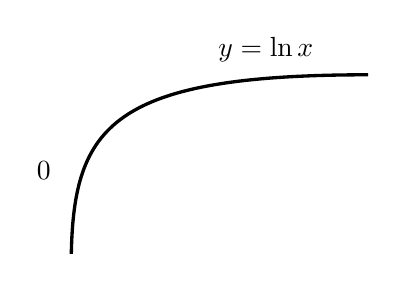
\begin{tikzpicture}[scale=0.65, thick]
			\tkzInit[xmin=-1, xmax=6, ymin=-2, ymax=3]
			\tkzDrawX \tkzDrawY
			\draw[very thick] (0.2, -2) .. controls (0.25, 0.5) and (1, 1.5) .. (6, 1.5) ;
			\node at (4, 2) {$y=\ln x$};
			\node[below left] at (0, 0) {$0$};
		\end{tikzpicture}
	\end{flushright}
\end{eg}
\textbf{Вывод}:
Вертикальные асимптоты ищем среди точек разрыва функции и граничных точек.
\newpage
\subsubsection{Наклонные асимптоты}
\begin{definition}\hlabel{опр: наклонная асимптота}
	Прямая $y=kx+b$ называется \textbf{наклонной асимптотой} графика функции $y=f(x)$ при $x \to \pm \infty$, если функция $f(x) = kx+b + \alpha(x)$, где $\alpha(x)$ --- б.м.ф. при $x\to \pm \infty$.
\end{definition}
\subsubsection{Горизонтальные асимптоты}
\begin{definition}
	Прямая $y=b$ называется \textbf{горизонтальной асимптотой} функции $y=f(x)$, если $\lim\limits_{x \to \pm \infty} f(x) = b$.
\end{definition}
\begin{corollary*}
	Горизонтальные асимптоты являются частным случаем наклонных асимптот при $k=0$.
\end{corollary*}

\subsection{Производная функции}

\begin{definition}\hlabel{опр: производная функции}
  \textbf{Производной функции $y = f(x)$} в точке $x_0$ называется \underline{предел} отношения приращения функции к приращению аргумента при стремлении последнего к нулю.
  \begin{align*}
    \boxed{y'(x_0) = \lim\limits_{\Delta x \to 0} \frac{\Delta y}{\Delta x}}
  \end{align*}
\end{definition}
\begin{definition}
  Производной функции $y=f(x)$ в точке $x_0$ справа(слева) или \textbf{правосторонней (левосторонней) производной} называется предел отношения приращения функции к приращению аргумента при стремлении к нулю справа(слева).
  \begin{gather*}
    \boxed{y'_+(x_0) = \lim\limits_{\Delta x \to 0+} \frac{\Delta y}{\Delta x}} \qquad \boxed{y'_-(x_0) = \lim\limits_{\Delta x \to 0-} \frac{\Delta y}{\Delta x}}
  \end{gather*}
\end{definition}
\begin{definition}
\textbf{Производной $\bm{n}$-го порядка} или \textbf{$\bm{n}$-ой производной} функции \\ $y=f(x)$ называется производная от $(n-1)$-ой производной функции $y=f(x)$
\begin{align*}
\boxed{y^{(n)} = \left( y^{(n-1)} \right)'}
\end{align*}
\end{definition}

\subsection{Дифференцируемая функция}

\begin{definition}\hlabel{опр: дифференцируемая функция}
  Функция $y=f(x)$ называется \textbf{дифференцируемой в точке} $\bm{x_0}$, если существует константа $A$ такая, что приращение функции в этой точке представимо в виде: \[ \boxed{\Delta y = A\cdot \Delta x + \alpha (\Delta x) \cdot \Delta x} \]
  где $\alpha (\Delta x)$ -- б.м.ф. при $\Delta x \to 0$
\end{definition}

\newpage
\subsection{Дифференциал первого порядка}

Пусть функция $y=f(x)$ определена в окрестности точки $x_0$ и дифференцируема в точке $x_0$.\\
Тогда по определению дифференцируемой функции: \begin{align}
	\Delta y = f'(x_0) \cdot \Delta x + \alpha (\Delta x) \cdot \Delta x
\end{align}
где $\alpha (\Delta x)$ -- б.м.ф. при $\Delta x \to 0$
\begin{definition}\hlabel{опр: дифференциал}
	\textbf{Дифференциалом} функции $y=f(x)$ в точке $x_0$ называется главная часть приращения функции $\Delta y$ или первое слагаемое в равенстве (1).
	\begin{align}
		\boxed{dy = f'(x_0) \cdot \Delta x}
	\end{align}
\end{definition}
\begin{note}\ \\ \vspace{-1.5\topsep}
  \begin{enumerate}
    \item Если $f'(x_0) = 0$, то $dy = 0$, но $f'(x_0) \cdot \Delta x$ уже не является главной частью приращения функции $\Delta y$.\\
    Пусть $y=x$, тогда по определению дифференциала $\Rightarrow\ dy = (x)' \cdot \Delta x = 1 \cdot \Delta x$. \\
    С другой стороны: $y = x\ \Rightarrow\ \boxed{dx = \Delta x}$\\
    \textbf{Вывод:} дифференциал независимой переменной равен её приращению.
    \item Подставим $\Delta x = dx$ в (2):
    \begin{align}
      \boxed{dy = f'(x_0)dx}
    \end{align} 
    Если $y=f(x)$ дифференцируема на интервале $(a;b)$, тогда $\forall x \in (a;b)\colon$
    \begin{align}
      &\boxed{dy = f'(x)dx}\\
      &\boxed{f'(x) = \frac{dy}{dx}}
    \end{align}
    \textbf{Вывод:} производная функции представима в виде отношения дифференциалов функции и независимой переменной.
  \end{enumerate}
\end{note}
\setcounter{equation}{0}

\begin{definition}
  $n$-ым дифференциалом или \textbf{дифференциалом $\bm{n}$-го порядка} называется дифференциал от дифференциала $(n-1)$-го порядка.
  \begin{gather*}
    d^ny = d(d^{n-1}y), \quad n=2,3,\ldots
  \end{gather*} 
\end{definition}

\subsection{Монотонные функции}\label{Монотонные функции}

\begin{definition}
	Функция $y=f(x)$, определённая на $(a;b)$, \textbf{возрастает} на этом интервале, если: \[ \forall\ x_1, x_2 \in (a;b)\colon x_2 > x_1\ \Rightarrow\ f(x_2) > f(x_1) \]
\end{definition}
\newpage
\begin{definition}\hlabel{опр: невозрастающая функция}
	Функция $y=f(x)$, определённая на $(a;b)$, \textbf{не возрастает} на этом интервале, если:
	\[ \forall\ x_1, x_2 \in (a;b)\colon x_2 > x_1\ \Rightarrow\ f(x_2) \le f(x_1) \]
\end{definition}

\begin{definition}
	Функция $y=f(x)$, определённая на $(a;b)$, \textbf{убывает} на этом интервале, если: \[ \forall\ x_1, x_2 \in (a;b)\colon x_2 > x_1\ \Rightarrow\ f(x_2) < f(x_1) \]
\end{definition}

\begin{definition}\hlabel{опр: неубывающая функция}
	Функция $y=f(x)$, определённая на $(a;b)$, \textbf{не убывает} на этом интервале, если:
	\[ \forall\ x_1, x_2 \in (a;b)\colon x_2 > x_1\ \Rightarrow\ f(x_2) \ge f(x_1) \]
\end{definition}

\begin{definition}
    Возрастающая, убывающая, невозрастающая и неубывающая функции называются \textbf{монотонными}.
\end{definition}

\begin{definition}
    Возрастающая и убывающая функции называются \textbf{строго монотонными}.
\end{definition}

\subsection{Минимумы, максимумы, экстремумы}

\begin{definition}
	Пусть $y=f(x)$ определена на $(a;b),\ x_0 \in (a;b)$. Тогда:\\[1ex]
	Если $\exists\ \mathring{S}(x_0),\ \forall x \in \mathring{S}(x_0)\colon f(x) \ge f(x_0)$, то \begin{tabular}{l} $x_0$ --- точка локального минимума, \\ $y_0 = y(x_0)$ --- \textbf{локальный минимум}. \end{tabular}
\end{definition}

\begin{definition}\hlabel{опр: строгий минимум}
	Пусть $y=f(x)$ определена на $(a;b),\ x_0 \in (a;b)$. Тогда:\\[1ex]
	Если $\exists\ \mathring{S}(x_0),\ \forall x \in \mathring{S}(x_0)\colon f(x) > f(x_0)$, то \begin{tabular}{l} $x_0$ -- \small{точка строгого локального минимума}, \\ $y_0 = y(x_0)$ -- \small{\textbf{строгий локальный минимум}}. \end{tabular}
\end{definition}

\begin{definition}
	Пусть $y=f(x)$ определена на $(a;b),\ x_0 \in (a;b)$. Тогда:\\[1ex]
	Если $\exists\ \mathring{S}(x_0),\ \forall x \in \mathring{S}(x_0)\colon f(x) \le f(x_0)$, то \begin{tabular}{l} $x_0$ --- точка локального максимума, \\ $y_0 = y(x_0)$ --- \textbf{локальный максимум}. \end{tabular}
\end{definition}

\begin{definition}\hlabel{опр: строгий максимум}
	Пусть $y=f(x)$ определена на $(a;b),\ x_0 \in (a;b)$. Тогда:\\[1ex]
	Если $\exists\ \mathring{S}(x_0),\ \forall x \in \mathring{S}(x_0)\colon f(x) < f(x_0)$, то\hspace{-2pt} \begin{tabular}{l} $x_0$ -- \small{точка строгого локального максимума}, \\ $y_0 = y(x_0)$ -- \small{\textbf{строгий локальный максимум}}. \end{tabular}
\end{definition}

\begin{definition}
    Минимум, максимум, строгий минимум, строгий максимум функции $f(x)$ называются \textbf{экстремумами} этой функции.
\end{definition}

\begin{definition}
    Строгий минимум и строгий максимум функции $f(x)$ называются \textbf{строгими экстремумами} этой функции.
\end{definition}

\newpage
\subsection{Стационарные и критические точки}

\begin{definition}
	Точки, в которых производная функции обращается в нуль, называются \textbf{стационарными}.
	\begin{gather*}
		f'(x_0) = 0\qquad x_0 \text{ --- стационарная точка}
	\end{gather*}
\end{definition}

\begin{definition}
	Точки, в которых производная функции обращается в нуль или не существует, называются \textbf{критическими точками 1-го порядка}.
\end{definition}

\begin{definition}
	Точки из области определения функции, в которых вторая производная функции равна нулю или не существует, называются \textbf{критическими точками 2-го порядка}.
\end{definition}

\subsection{Выпуклость (вверх или вниз) графика функции на промежутке}

\begin{definition}\hlabel{опр: выпуклая функция}
    Пусть функция $f(x)$ определена на интервале $(a;b)$. Функция $f(x)$ называется \textbf{выпуклой вверх (вниз)} на этом интервале, если любая точка касательной, проведённой к графику функции $f(x)$ (кроме точки касания) лежит выше (ниже) точки графика функции $f(x)$ с такой же абсциссой.
\end{definition}

\subsection{Точка перегиба графика функции}

\begin{definition}\hlabel{опр: точка перегиба}
    Пусть функция $f(x)$ определена на интервале $(a;b)$.\\
    Точка $x_0 \in (a;b)$ называется \textbf{точкой перегиба \underline{функции}} $f(x)$, если эта функция непрерывна в точке $x_0$ и если существует число $\delta > 0$ такое, что направление выпуклости функции $f(x)$ на интервалах $(x_0 - \delta; x_0)$ и $(x_0; x_0 + \delta)$ различны.\\
    При этом точка $\big(x_0, f(x_0)\big)$ называется \textbf{точкой перегиба \underline{графика функции}} $f(x)$.
\end{definition}

\newpage
\section{Используемые теоремы}

\begin{theorem}[О существовании предела функции в точке]\hlabel{существование предела в точке}
  Функция $y = f(x)$ в точке  $x_0$ имеет конечный предел тогда и только тогда, когда существуют пределы справа и слева и они равны между собой.
  \begin{gather*}
    \lim_{x \to x_0} f(x) = \lim_{x \to x_0+} f(x) = \lim_{x \to x_0-} f(x) 
  \end{gather*}
\end{theorem}

\begin{theorem}[О сумме конечного числа бесконечно малых функций] \hlabel{о сумме конечного числа б.м.ф.}
  Конечная сумма бесконечно малых функции есть бесконечно малая функция.
\end{theorem}
% \begin{proof}
%   Пусть дано конечное число бесконечно малых функций, например: $\alpha(x), \beta(x), x\to x_0$.
%   Тогда по определению бесконечно малой функции (\textbf{опр.\ref{опр: б.м.ф.}}): 
%   \[
%   \lim_{x \to x_0} \alpha(x) = 0 \qquad \lim_{x \to x_0} \beta(x) = 0
%   \]
%   Нужно доказать, что: $\lim\limits_{x \to x_0} \big(\alpha(x) + \beta(x)\big) = 0$ \\
%   Распишем: 
%   \begin{gather*}
%     \lim_{x \to x_0} \alpha(x) = 0 \iff \left(\forall \varepsilon_1 = \frac{\varepsilon}{2} > 0\right)\big(\exists \delta_1 > 0\big)\colon \left(\forall x \in \mathring{S}(x_0; \delta_1) \Rightarrow\ |\alpha(x)| < \varepsilon_1 = \frac{\varepsilon}{2}\right) \tag{1}\\
%     \lim_{x \to x_0} \beta(x) = 0 \iff \left(\forall \varepsilon_2 = \frac{\varepsilon}{2} > 0\right)\big(\exists \delta_2 > 0\big)\colon \left(\forall x \in \mathring{S}(x_0; \delta_2) \Rightarrow\ |\beta(x)| <  \varepsilon_2 = \frac{\varepsilon}{2}\right) \tag{2}
%   \end{gather*}
%   Выберем $\delta = \min \{\delta_1; \delta_2\}$. Тогда (1) и (2) верны одновременно. Получаем:
%   \begin{gather*}
%     \big(\forall \varepsilon > 0\big)\big(\exists \delta > 0\big)\colon \left(\forall x \in \mathring{S}(x_0; \delta) \Rightarrow\ |\alpha(x) + \beta(x)| \le |\alpha(x)| + |\beta(x)| < \frac{\varepsilon}{2} + \frac{\varepsilon}{2} = \varepsilon\right) 
%   \end{gather*}
%   Тогда по определению бесконечно малой функции:
%   \[
%   \lim_{x \to x_0} \big(\alpha(x) + \beta(x)\big) = 0
%   \] 
% \end{proof}

\begin{theorem}\hlabel{для непрерывности сложной функции}
  Пусть функция $g(y)$ непрерывна в точке $y_0$, $y_0 = \lim\limits_{x\to x_0}f(x)$.\\
  Тогда $\lim\limits_{x\to x_0}g(f(x)) = g\left(\lim\limits_{x\to x_0}f(x)\right)$
\end{theorem}

\begin{theorem}[О существовании производной функции в точке]\hlabel{Существование производной функции в точке}
  Функция $y = f(x)$ в точке $x_0$ имеет производную тогда и только тогда, когда она имеет производные и справа, и слева, и они равны между собой.
  \begin{align*}
    y'(x_0) = y'_+(x_0)=y'_-(x_0)
  \end{align*}
\end{theorem}

\setcounter{equation}{0}
\begin{theorem}\hlabel{формула Тейлора}
	Пусть функция $y=f(x)$ $n$ раз дифференцируема в точке $x_0$ и определена в некоторой окрестности этой точки. Тогда $\forall x \in S(x_0)$ имеет место формула Тейлора:
	\begin{align}
		\begin{aligned}
			f(x) =& f(x_0)  + \frac{f'(x_0)}{1!}\cdot (x-x_0) + \frac{f''(x_0)}{2!}\cdot (x-x_0)^2 + \frac{f'''(x_0)}{3!}\cdot (x-x_0)^3 + \\
			              & + \ldots + \frac{f^{(n)}(x_0)}{n!}\cdot (x-x_0)^n + R_n(x)
		\end{aligned}
	\end{align}
	Кратко: $f(x) = P_n(x) + R_n(x)$, где
	\begin{flalign*}
		&\begin{aligned}
		P_n(x) =& f(x_0)  + \frac{f'(x_0)}{1!}\cdot (x-x_0) + \frac{f''(x_0)}{2!}\cdot (x-x_0)^2 + \frac{f'''(x_0)}{3!}\cdot (x-x_0)^3 + \\
		& + \ldots + \frac{f^{(n)}(x_0)}{n!}\cdot (x-x_0)^n \hspace{2cm} \text{--- многочлен Тейлора}\qquad x\to x_0
		\end{aligned}  &
	\end{flalign*}
	$R_n(x)$ --- остаточный член формулы Тейлора
\end{theorem}

\newpage
\section{Дополнительно}
\begin{table}[h]
  \centering
  \caption{Таблица эквивалентных б.м.ф.}
  \begin{tabular}{|ll|}
    \hline
    1. $\sin x \sim x$ при $x\to 0$; &\quad 6. $e^x - 1 \sim x\ (x \to 0)$;\\
    2. $\tg x \sim x\ (x \to 0)$; &\quad 7. $a^x - 1 \sim x \cdot \ln a\ (x \to 0)$;\\
    3. $\arcsin x \sim x\ (x \to 0)$; &\quad 8. $\ln(1 + x) \sim x\ (x \to 0)$;\\
    4. $\arctg x \sim x\ (x \to 0)$; &\quad 9. $\log_a (1 + x) \sim x\cdot \log_a e\ (x \to 0)$;\\
    5. $1 - \cos x \sim \dfrac{x^2}{2}\ (x \to 0)$; &\quad 10. $(1 + x)^k - 1 \sim k\cdot x,\ k>0\ (x \to 0)$;\\
    \multicolumn{2}{|l|}{11. $a_0 + a_1x + a_2x^2 + \ldots + a_nx^2 \sim a_nx^2\ (x \to \infty)$} \\
    \multicolumn{2}{|l|}{12. $a_1x + a_2x^2 + \ldots + a_nx^n \sim a_1x\ (x \to 0)$} \\
    \hline
  \end{tabular}
\end{table}

\begin{table}[h]
  \centering
  \caption{Формулы дифференцирования}
  \begin{tabular}{|ll|}
    \hline
    \vspace{-7pt} & \\
    \multicolumn{2}{|l|}{1. $(c)'=0$;}\\
    \multicolumn{2}{|l|}{2. $\left(u^a\right)'=a \cdot u^{a - 1}\cdot u'$, в частности, $(\sqrt{u})'=\dfrac{1}{2\sqrt{u}}\cdot u'$;}\\[1ex]
    \multicolumn{2}{|l|}{3. $\left(a^u\right)'=a^u\cdot \ln a \cdot u'$, в частности, $(e^u)'=e^u\cdot u'$;}\\
    \multicolumn{2}{|l|}{4. $\left(\log_a u\right)' = \dfrac{1}{u \cdot \ln a}\cdot u'$, в частности, $(\ln u)' = \dfrac{1}{u}\cdot u'$;}\\[2ex]
    5. $(\sin u)' = \cos u \cdot u';$ & 6. $(\cos u)' = -\sin u \cdot u'$;\\[1ex]
    7. $(\tg u)' = \dfrac{1}{\cos^2 u}\cdot u';$ & 8. $(\ctg u)' = -\dfrac{1}{\sin^2 u} \cdot u'$;\\[2ex]
    9. $(\arcsin u)' = \dfrac{1}{\sqrt{1 - u^2}}\cdot u'$; & 10. $(\arccos u)' = -\dfrac{1}{\sqrt{1 - u^2}}\cdot u'$;\\[2ex]
    11. $(\arctg u)' = \dfrac{1}{1+u^2}\cdot u'$; & 12. $(\arcctg u)' = -\dfrac{1}{1+u^2}\cdot u'$;\\[2ex]
    13. $(\sh u)' = \ch u \cdot u'$; & 14. $(\ch u)' = \sh u \cdot u'$;\\[1ex]
    15. $(\th u)' = \dfrac{1}{\ch^2 u} \cdot u'$; & 16. $(\cth u)' = -\dfrac{1}{\sh^2 u} \cdot u'$.\\[2ex]
    \hline
  \end{tabular}
\end{table}

\end{document}